%!TEX TS-program = pdflatex
%!TEX encoding = UTF-8 Unicode
% =============================================================================
%  P1_bernoulli_20260701_Bernoulli_revised.tex   --  Bernoulli submission version
%  Compile order:
%    (1) pdflatex P1_bernoulli_supp_20260701_Bernoulli_revised.tex   (twice)
%    (2) pdflatex P1_bernoulli_20260701_Bernoulli_revised.tex
%    (3) bibtex   P1_bernoulli_20260701_Bernoulli_revised
%    (4) pdflatex P1_bernoulli_20260701_Bernoulli_revised.tex  (twice)
% =============================================================================
\documentclass[bj,authoryear]{imsart}

\usepackage{amsmath,amssymb,mathtools}
\usepackage{bm}
\usepackage{booktabs}
\usepackage{array}
\usepackage{multirow}
\usepackage{enumitem}
\usepackage{graphicx}
\usepackage{float}
\usepackage[section]{placeins}
\usepackage{microtype}
% ── Local definitions (theorem environments + math macros) ───────────────────
\startlocaldefs
\emergencystretch=2em

\theoremstyle{plain}
\newtheorem{theorem}{Theorem}[section]
\newtheorem{proposition}[theorem]{Proposition}
\newtheorem{lemma}[theorem]{Lemma}
\newtheorem{corollary}[theorem]{Corollary}
\theoremstyle{definition}
\newtheorem{definition}[theorem]{Definition}
\newtheorem{example}[theorem]{Example}
\newtheorem{remark}[theorem]{Remark}
\newtheorem{assumption}[theorem]{Assumption}

\newcommand{\E}{\mathbb{E}}
\newcommand{\Prob}{\mathbb{P}}
\newcommand{\R}{\mathbb{R}}
\newcommand{\N}{\mathbb{N}}
\newcommand{\F}{\mathcal{F}}
\newcommand{\G}{\mathcal{G}}
\newcommand{\A}{\mathcal{A}}
% \Z intentionally undefined (use \mathbb{Z} for integers, \mathcal{Z} directly for scores)
\newcommand{\Tsig}{\mathcal{T}_\infty}
\newcommand{\norm}[1]{\left\lVert #1 \right\rVert}
\newcommand{\abs}[1]{\left| #1 \right|}
\newcommand{\inner}[2]{\langle #1,\, #2 \rangle}
\newcommand{\given}{\mid}
\newcommand{\iid}{\overset{\mathrm{iid}}{\sim}}
\DeclareMathOperator{\Var}{Var}
\DeclareMathOperator{\Cov}{Cov}
\DeclareMathOperator*{\argmin}{arg\,min}
\newcommand{\od}[1]{\overset{d}{#1}}

\endlocaldefs

%% Cross-references to the companion document are LIVE and SELF-FREEZING.
%% While the companion's .aux is present it is read at compile time (only
%% its \newlabel entries are kept), so renumbering can never go stale, and
%% a snapshot \jobname-xrefs.tex is (re)written automatically on every
%% compile.  When the companion's .aux is absent -- e.g. the journal
%% compiling this file in isolation -- the snapshot is used instead.
%% Submission: upload \jobname-xrefs.tex together with the source, exactly
%% like the .bbl file.  (The xr package is NOT used: imsart forbids it.)
\makeatletter
\newwrite\companion@xrefs@out
\newcommand{\companionlabel}[2]{%
  \global\expandafter\def\csname r@#1\endcsname{#2}}
\def\companion@readaux#1{%
  \immediate\openout\companion@xrefs@out=\jobname-xrefs.tex
  \immediate\write\companion@xrefs@out{%
    \@percentchar\space Snapshot of the cross-references in #1.aux.}%
  \immediate\write\companion@xrefs@out{%
    \@percentchar\space Auto-regenerated on every compile; do not edit.}%
  \begingroup
    \let\citation\@gobble
    \let\bibdata\@gobble
    \let\bibstyle\@gobble
    \def\bibcite##1##2{}%
    \long\def\@writefile##1##2{}%
    \def\newlabel##1##2{%
      \companionlabel{##1}{##2}%
      \immediate\write\companion@xrefs@out{%
        \string\companionlabel{##1}{\unexpanded{##2}}}}%
    \@@input #1.aux\relax
  \endgroup
  \immediate\closeout\companion@xrefs@out}
\def\companion@fallback#1{%
  \IfFileExists{\jobname-xrefs.tex}%
    {\typeout{** #1.aux not found; using frozen snapshot \jobname-xrefs.tex}%
     \input{\jobname-xrefs.tex}}%
    {\typeout{** #1.aux not found and no snapshot; companion refs undefined}}}
\newcommand{\inputcompanionaux}[1]{%
  \IfFileExists{#1.aux}%
    {\companion@readaux{#1}}%
    {\companion@fallback{#1}}}
\inputcompanionaux{P1_bernoulli_supp_20260701_Bernoulli_revised}
\makeatother

% =============================================================================
\begin{document}

\begin{frontmatter}

\title{Martingale Innovations from Recurrent Networks
       for Sequential Change-Point Detection}
\runtitle{Martingale Innovations for Change-Point Detection}

\author{\inits{Y.-C.\,I.}\fnms{Yuan-chin Ivan}~\snm{Chang}%
  \ead[label=e1]{ycchang@sinica.edu.tw}}
\address{Institute of Statistical Science, Academia Sinica,
  128 Academia Road, Section~2, Nankang, Taipei 115, Taiwan.
  \printead[presep={\ }]{e1}}

\begin{abstract}
Sequential monitoring is difficult when observations are serially
dependent, high-dimensional, and lack a trusted parametric model.  This
paper revisits the innovations principle with a learned predictor: a
recurrent network removes the serially predictable component of the stream,
and a CUSUM statistic monitors the resulting prediction innovations.  Its aim
is foundational: the false-alarm and delay guarantees of classical
change-point theory carry over, essentially intact, to a black-box learned
predictor.  The development is two-tier.  First, for contractive recurrent
networks, the hidden state admits a Doob decomposition into a predictable
part and a martingale-difference innovation that stabilizes geometrically
and whose partial sums obey a functional central limit theorem.  Second, for
any predictor with an almost-sure bound on the conditional residual drift and
sub-Gaussian tails, the Innovation CUSUM has an exponential lower bound on the
in-control average run length---with the best exponent available uniformly over
that class---and a logarithmic upper bound on the detection delay.  In the
Gaussian mean-shift case the statistic coincides with the classical
likelihood-ratio CUSUM and is first-order minimax optimal.  The guarantee needs
no parametric model for the observed dynamics, though it is not assumption-free;
we also give conditions under which a learning guarantee verifies the drift
condition with high probability.  We also identify when learning helps: under a nonlinear
conditional mean, linear residualization has an irreducible defect that a
learned predictor removes.  Simulations and real-data examples illustrate the
theory.
\end{abstract}

\begin{keyword}
\kwd{martingale decomposition}
\kwd{recurrent neural network}
\kwd{LSTM}
\kwd{change-point detection}
\kwd{CUSUM}
\kwd{average run length}
\kwd{dimension stability}
\kwd{locally stationary processes}
\end{keyword}

\begin{keyword}[class=MSC]
\kwd[Primary ]{62L10}
\kwd{60G42}
\kwd[; secondary ]{62M10}
\kwd{62M45}
\end{keyword}

\end{frontmatter}

\section{Introduction}
\label{sec:intro}

Streams of data that must be monitored for structural change are now routine: intensive-care units track dozens of physiological signals, public-health agencies monitor infectious-disease incidence, industrial systems log hundreds of correlated sensor channels, and risk desks follow panels of asset returns. In each case, a detector must decide online whether the mechanism generating the stream has changed. The two possible errors have different costs. A \emph{false alarm} --- firing while the system remains in control --- may trigger an unnecessary clinical intervention, halt a production line, or prompt a premature portfolio rebalancing. A \emph{missed detection}, or a long detection delay, may leave a deteriorating patient unmonitored, an equipment fault undetected, or a loss unhedged. The statistical problem is therefore not merely to detect change, but to control false alarms without paying for that control through excessive delay.

This trade-off is especially difficult in the settings that motivate this paper. The observations are serially dependent; the dependence structure is typically unknown in advance and rarely specified with enough confidence to support a parametric monitor; and the number of monitored coordinates may be large. Sequential change-point detection under these three conditions --- unknown serial dependence, limited model specification, and growing dimension --- is the problem studied here.

Several commonly used tools solve parts of this problem. Classical CUSUM procedures are powerful --- indeed optimal --- under independence or a correctly specified parametric model
\citep{page1954continuous,lorden1971procedures}, while offline segmentation
\citep{killick2012optimal} and Bayesian online methods
\citep{adams2007bayesian} offer flexible alternatives. These approaches, however, generally lose their false-alarm guarantees once the serial dependence structure is unknown or the observation dimension grows. Classical time-series models handle dependence explicitly: autoregressive models fix the lag order, hidden Markov models encode memory through a finite state space, and Kalman filters propagate a Gaussian sufficient statistic
\citep{box2015time,hamilton1994time}. They inherit clean guarantees when the model is correct, but only at the price of requiring the model to be correct. What is missing is a monitoring scheme whose false-alarm behavior remains valid under unknown serial dependence and growing dimension.

A further strand of literature monitors \emph{residuals} rather than raw
observations.  Monitoring with estimated parameters goes back at least to
\citet{chu1996monitoring}; the asymptotics of sequential residual
empirical processes were developed by \citet{bai1994residuals};
\citet{lai1995sequential} treats sequential detection in dynamical
systems; and \citet{aue2013structural} survey structural-break detection
for time series.  These procedures monitor the residuals of a
\emph{specified} parametric class, and their guarantees are tied to that
class being correct.  In a complementary direction, conformal test
martingales and e-detectors \citep{vovk2005algorithmic,shin2024edetectors}
provide anytime-valid nonparametric monitoring under exchangeability-type
conditions or a known in-control reference.  The present paper sits
between the two strands: like the residual tradition it monitors one-step
prediction errors, but the predictor is learned rather than specified;
like the e-detector tradition it avoids a parametric model of the
dynamics, but the in-control requirement is an explicit residual
drift-and-tail condition rather than exchangeability, and the monitor is
the classical Page CUSUM.

This paper takes a route with a long pedigree in time-series analysis:
transform the observations into innovations, then monitor the innovations.
The innovations principle --- that the one-step prediction error of an
optimal predictor carries no serially predictable component --- underlies
Wiener--Kolmogorov prediction theory, the innovations approach to filtering
\citep{kailath1968innovations}, residual diagnostics in Box--Jenkins
modeling \citep{box2015time}, and residual-based detection of abrupt
changes \citep{basseville1993detection}. In the linear-Gaussian world the
principle is exact: Kalman-filter innovations are independent, and a CUSUM
applied to them inherits the classical false-alarm guarantees. Outside
that world, however, the filter must be specified correctly --- precisely
what is unavailable when the dependence structure is unknown. Recurrent
neural networks (RNNs) \citep{rumelhart1986learning}, long short-term
memory networks (LSTMs) \citep{hochreiter1997long}, gated recurrent units
(GRUs) \citep{cho2014learning}, and selective state-space models such as
Mamba \citep{gu2023mamba} learn predictive state representations from data
rather than fixing the memory structure in advance. They therefore supply
a natural modern implementation of the innovations principle: use a learned
predictor to remove the serially predictable component, and monitor what
remains. The question this paper answers is what survives of the classical
CUSUM guarantees when the filter is learned rather than specified.

Two questions must be answered. First, in what precise probabilistic sense
does a learned recurrent state generate innovations, and how quickly do
those innovations stabilize, so that calibration performed on a training
segment remains valid at monitoring time? Second, what sequential-monitoring
guarantee does a CUSUM applied to learned innovations inherit, and does
that guarantee withstand growing observation dimension?

Our answers are deliberately two-tier. At the first tier, for the basic
RNN recurrence under an operator-norm contraction condition on the recurrent
weight matrix (Assumption~\ref{ass:spectral}) --- a condition the
practitioner can \emph{enforce} through spectral normalization
\citep{miyato2018spectral} rather than merely hope for --- the hidden state
admits a classical Doob decomposition into a predictable component and a
martingale-difference innovation. The innovation converges geometrically
to its stationary counterpart, and the accumulated innovations obey a
functional central limit theorem.

At the second tier, the detector's guarantee is architecture-agnostic by
design. Exact Bayes prediction residuals are martingale differences
(Proposition~\ref{prop:predresid}); fitted residuals are useful to the
extent that their conditional mean drift is small.  The contractive-RNN
result supports this condition through a bridge bound
(Proposition~\ref{prop:rnn-resid-bridge}), which separates three sources of
error: transient hidden-state initialization, readout approximation to the
Bayes predictor, and estimation error.  The CUSUM theory itself then assumes
directly that the fitted residuals have bounded conditional drift and
conditional sub-Gaussian tails.  Under those operating conditions it yields
an in-control average-run-length lower bound
(Theorem~\ref{thm:arl}) and an out-of-control detection-delay upper bound
(Theorem~\ref{thm:delay}), which together give the
exponential-false-alarm / logarithmic-delay trade-off
(Corollary~\ref{cor:tradeoff}).  Thus the RNN stabilization theorem
motivates and partially verifies the residual condition, while the CUSUM
guarantee applies to any learned predictor satisfying that condition.

The contributions organize around four connected claims. First, under
operator-norm contractivity, recurrent hidden states generate stabilized
martingale-difference innovations: the hidden state is uniformly
$L^2$-bounded, decomposes into a predictable component plus an innovation,
and the innovation converges geometrically to its stationary counterpart
(Theorem~\ref{thm:mds}). The accumulated innovations then satisfy a
martingale functional central limit theorem
(Corollary~\ref{cor:fclt}). Second, a new bridge proposition translates this
state-level stabilization into a residual-level approximation bound for
recurrent predictors with Lipschitz readouts
(Proposition~\ref{prop:rnn-resid-bridge}). Third, for fitted prediction
residuals satisfying explicit conditional-drift and tail assumptions, the
Innovation CUSUM has a sharp exponential in-control average-run-length lower
bound and a corresponding out-of-control detection-delay upper bound
(Theorems~\ref{thm:arl} and~\ref{thm:delay}); together they attain the
minimax-optimal detection \emph{rate} of classical sequential analysis, and in
the Gaussian mean-shift case the analytic threshold is first-order minimax
optimal, with exact Lorden optimality holding for the Page CUSUM calibrated to
the false-alarm constraint (Theorem~\ref{thm:optimality}). Fourth, we identify
\emph{when} learning helps: under a nonlinear conditional mean, any fixed
linear residualization carries an irreducible innovation defect, whereas a
consistent learned predictor drives this defect to zero
(Proposition~\ref{prop:whiteness}), improving the guaranteed in-control ARL
through the drift margin (Remark~\ref{rem:whiteness-arl}).  The empirical
studies then examine these mechanisms: learned innovations are closer to
martingale differences under misspecification, calibration is more stable
when the in-control window is short, and equal-ARL comparisons delimit when
the learned detector is competitive with correctly specified parametric
procedures.

The contribution lies in this synthesis. The individual ingredients are
classical --- the Doob decomposition of an adapted square-integrable
process; the martingale-difference property of Bayes prediction residuals;
the geometric forgetting of initial conditions under a contractive
stochastic recursion, standard in iterated-random-function and mixing
theory \citep{doukhan1994mixing} and used elsewhere for stable recurrent
models \citep{miller2019stable}; the martingale functional central limit
theorem \citep{hall1980martingale,billingsley1999convergence}; the
$L^2$-orthogonal-projection characterization of the best linear predictor
(Proposition~\ref{prop:whiteness}); and CUSUM theory dating to
\citet{page1954continuous} and \citet{lorden1971procedures}, including the
exponential-supermartingale argument used for its false-alarm guarantee.
None of these building blocks is new on its own. What appears to be new is
their combination:
using contractive recurrent states to construct stabilized innovation
processes, connecting these innovations to fitted prediction residuals,
and deriving a nonparametric sequential-monitoring guarantee for the
resulting approximate-MDS CUSUM under explicit residual-drift and tail
conditions.

This perspective is distinct from most existing theory for recurrent
architectures, which emphasizes stability or expressivity
\citep{miller2019stable,miyato2018spectral,gonon2020reservoir}, and from
neural tangent kernel and information-bottleneck analyses, which primarily
concern feedforward networks or fixed-time representations
\citep{jacot2018neural,tishby2015deep,saxe2019information}. Structured
state-space models such as Mamba
\citep{gu2021efficiently,gu2023mamba} have likewise been studied mainly
from the standpoint of efficient sequence modeling
\citep{orvieto2023resurrecting}. Here the focus is different: the learned
state is used to remove the serially predictable component of the stream,
so that the remaining innovation process can be monitored with
model-free sequential guarantees under explicit drift, tail, and
post-change signal assumptions.

The theoretical framework and main results appear in
Sections~\ref{sec:theory}--\ref{sec:pathway}, followed by four empirical
studies in Section~\ref{sec:empirical}. Eight additional studies,
background definitions, and all formal proofs are given in the
Supplementary Material. Table~\ref{tab:assumption-map} summarizes the
assumptions and conclusions of the main results and makes explicit the
two-tier structure of the paper: contractive-RNN innovation theory in
Section~\ref{sec:theory} and architecture-agnostic detection theory in
Section~\ref{sec:pathway}.

% =============================================================================
\section{Methodology}
\label{sec:theory}

%\subsection*{Setup}

We work on a complete probability space $(\Omega, \mathcal{A}, \mathbb{P})$.
Let $(X_t)_{t\geq 1}$ be a strictly stationary ergodic process; by
Kolmogorov's extension theorem we may, and do, extend it to a two-sided
strictly stationary ergodic process $(X_t)_{t\in\mathbb{Z}}$.
Throughout Sections~\ref{sec:theory}--\ref{sec:pathway} the filtration is
the \emph{two-sided} natural filtration
$\mathcal{F}_t=\sigma(X_s:s\leq t)\vee\sigma(h_0)$, $t\in\mathbb{Z}$,
where the RNN initial state $h_0$ (introduced below) is square-integrable
and independent of $(X_t)_{t\in\mathbb{Z}}$; a deterministic $h_0$, as in
all our experiments, is a special case.  Conditioning on the two-sided
past is what makes the stationary innovation process of
Section~\ref{sec:rnn-decomp} exactly stationary and adapted; the detector
of Section~\ref{sec:pathway} conditions only on the observable one-sided
history, and its guarantees are self-contained there.
The tail $\sigma$-algebra is
$\Tsig = \bigcap_{t\geq 1}\sigma(X_t, X_{t+1},\ldots)$.
Throughout Sections~\ref{sec:theory}--\ref{sec:pathway} we use $p$ to denote the hidden-state dimension and $d_{\mathrm{in}}$ for the input dimension.
An RNN processes the sequence via $h_t = \phi(W_h h_{t-1} + W_x x_t + b_h)$ (with $h_t\in\R^p$)
and an LSTM augments this with a gated cell state; both architectures are
defined precisely in Section~\ref{app:background} of the Supplementary Material.
In Section~\ref{sec:empirical} the symbol $d$ refers to the
observation (input) dimension of the multivariate DGP, following the
change-point literature convention.
Throughout, we assume the effective recurrent Lipschitz constant satisfies
$L_\phi\|W_h\|_{\mathrm{op}} < 1$ (operator-norm contractivity;
see Assumption~\ref{ass:spectral} below),
which can be encouraged in practice by spectral normalization
\citep{miyato2018spectral}.
For one-step prediction of a target $Y_{t+1}$, the central object is the
innovation $e_{t+1}=Y_{t+1}-\E[Y_{t+1}\mid\mathcal F_t]$, whose
martingale-difference sequence (MDS) property is stated in
Proposition~\ref{prop:predresid}.
A process $(X_t)$ is \emph{absolutely regular} ($\beta$-mixing) if its
mixing coefficients
$\beta(k)=\sup_t\E\{\sup_{B\in\sigma(X_{t+k},X_{t+k+1},\ldots)}
|\Prob(B\mid\F_t)-\Prob(B)|\}$ tend to zero.  Such assumptions are used only
for empirical motivation and local approximation, not to claim that $(h_t)$
alone is a Markov chain.
Full definitions, the reverse martingale convergence theorem, and the
i.i.d. Hewitt--Savage zero-one law are collected in Section~\ref{app:background} of the Supplementary Material.

\begin{remark}[Non-tail-measurable targets]
\label{rem:nontail}
  Parts~(d)--(e) of Lemma~\ref{lem:equiv} (Supplementary Material) show that
  when the target $\theta$ is not tail-measurable,
  the forward and reverse limits \emph{differ}: the forward limit
  $\E[\theta\given\F_\infty^+]$ may incorporate information from the finite
  initial segment, while the reverse limit $\E[\theta\given\Tsig]$ discards it.
  This formalizes \emph{selective forgetting}: the reverse martingale extracts
  only the structurally persistent (tail-measurable) component of any target.
\end{remark}


\begin{assumption}[Effective operator-norm contractivity]
\label{ass:spectral}
  Throughout the paper we assume $L_\phi\norm{W_h}_{\mathrm{op}}<1$,
  where $L_\phi$ is the Lipschitz constant of $\phi$ and
  $\norm{W_h}_{\mathrm{op}}=\sigma_{\max}(W_h)$.
  Spectral normalization \citep{miyato2018spectral} can encourage this
  condition in practice.
\end{assumption}

\subsection{Martingale Decomposition of RNN Hidden States}
\label{sec:rnn-decomp}

Throughout this subsection we work under Assumption~\ref{ass:spectral}
($\rho:=L_\phi\norm{W_h}_{\mathrm{op}}<1$).
The existence and uniqueness of the stationary causal solution
$(H_t^*)_{t\in\mathbb{Z}}$ satisfying
$H_t^*=\phi(W_hH_{t-1}^*+W_xX_t+b_h)$,
$H_t^*\in\sigma(X_t,X_{t-1},\ldots)$,
and the geometric coupling bound
$\norm{h_t-H_t^*}_{L^2}\leq\rho^t\norm{h_0-H_0^*}_{L^2}$
are proved directly in Proposition~\ref{prop:stationary-causal}
(Section~\ref{app:stationary-causal} of the Supplementary Material), so this
paper's theorem chain does not depend on any external or unpublished result.
The companion paper \citet{chang2026backward} studies the complementary question
of hidden-state convergence under the same contraction condition from a
reverse-filtration perspective; none of its results are used here.
We write $\Delta_0:=\norm{h_0-H_0^*}_{L^2}$,
$D_t^*:=\E[H_t^*\given\F_{t-1}]$ (stationary predictable component),
and $M_t^*:=H_t^*-D_t^*$ (stationary MDS innovation).
Here the two-sided filtration of the setup is essential: $H_t^*$ is a
fixed measurable functional of $(X_s)_{s\leq t}$, hence
$\F_t$-measurable, and $D_t^*$ is the same functional of the shifted path
at every $t$ (conditioning on the independent $\sigma(h_0)$ leaves it
unchanged), so $(M_t^*)_{t\in\mathbb{Z}}$ is a strictly stationary,
ergodic MDS \emph{adapted} to $(\F_t)$.  With the one-sided filtration
$\sigma(X_1,\ldots,X_{t-1})$ neither exact stationarity nor adaptedness
would hold, because the pre-sample past influences $H_t^*$.
The stationary causal solution is generally a \emph{random} process;
it should not be identified with a deterministic mean-field fixed point
or a tail projection.

The Doob decomposition in part~(ii) of the following theorem is, on its
own, elementary: subtracting its conditional expectation turns any
square-integrable adapted process into a predictable term plus a
martingale difference.  The substance of Theorem~\ref{thm:mds} is what the
contractive recursion adds to this decomposition --- uniform $L^2$ control,
the \emph{geometric stabilization} of the innovation toward its stationary
counterpart (iv), and the stationary innovation covariance $\Sigma_M^*$
(v) --- which are the ingredients the functional CLT
(Corollary~\ref{cor:fclt}) and the Innovation CUSUM
(Section~\ref{sec:pathway}) actually consume.

\begin{theorem}[MDS Decomposition with Stabilization Rate]
\label{thm:mds}
  Let $(X_t)_{t\geq 1}$ be a strictly stationary ergodic process with
  $\E\norm{X_t}^2<\infty$, and let $(h_t)_{t\geq 0}$ be the RNN
  hidden-state sequence with initial state $h_0$ as in the setup
  (square-integrable, independent of the process).
  Set $\rho=L_\phi\norm{W_h}_{\mathrm{op}}<1$ and
  $\Delta_0=\norm{h_0-H_0^*}_{L^2}$.  Then, for each $t\geq 2$:
  \begin{enumerate}[label=(\roman*), itemsep=3pt]
    \item \textbf{($L^2$-boundedness.)}
      $(h_t)$ is uniformly $L^2$-bounded.  When $\phi(0)=0$ (e.g.\ $\tanh$, ReLU):
      \[
        \sup_t\norm{h_t}_{L^2}
        \leq \norm{h_0}_{L^2}
          +\frac{L_\phi\bigl(\norm{W_x}_{\mathrm{op}}\norm{X_1}_{L^2}
                  +\norm{b_h}\bigr)}{1-\rho}
        =: C_0 < \infty.
      \]
      For activations with $\phi(0)\neq 0$ (e.g.\ sigmoid), an additional term $\|\phi(0)\|/(1-\rho)$ is added to $C_0$ (from $\|\phi(u)\|\leq\|\phi(0)\|+L_\phi\|u\|$, so the constant enters undamped by $L_\phi$); finiteness is unchanged.
    \item \textbf{(MDS decomposition.)}
      The Doob decomposition $h_t=D_t+M_t$ holds, where
      $D_t:=\E[h_t\given\F_{t-1}]$ is $\F_{t-1}$-measurable (predictable)
      and $M_t:=h_t-D_t$ satisfies $\E[M_t\given\F_{t-1}]=0$ a.s.
      The pair $(M_t,\F_t)_{t\geq 2}$ is a martingale difference sequence.
    \item \textbf{(Innovation $L^2$ bound.)}
      Writing $\Var_2(X_t):=\E\norm{X_t-\E X_t}^2$,
      \begin{equation}
        \E\norm{M_t}^2
        \leq L_\phi^2\norm{W_x}_{\mathrm{op}}^2\Var_2(X_t)
        =: \sigma_M^2.
        \label{eq:Mbound}
      \end{equation}
    \item \textbf{(Innovation stabilization rate.)}
      The MDS innovations converge to their stationary counterparts
      at a geometric rate:
      \begin{equation}
        \norm{M_t-M_t^*}_{L^2} \leq 2\rho^t\Delta_0.
        \label{eq:Mstab}
      \end{equation}
    \item \textbf{(Conditional variance decomposition and stationary
          innovation covariance.)}
      The law-of-total-variance decomposition holds exactly:
      \begin{equation}
        \E\norm{h_t-\E h_t}^2
        = \E\norm{D_t-\E h_t}^2 + \E\norm{M_t}^2.
        \label{eq:var-decomp}
      \end{equation}
      In the stationary regime the innovation covariance matrix
      \begin{equation}
        \Sigma_M^* := \E\bigl[M_t^*\,(M_t^*)^\top\bigr]
        \label{eq:SigmaM}
      \end{equation}
      is well-defined, independent of $t$, positive semi-definite,
      and satisfies $\Sigma_M^* \preceq \sigma_M^2 I_p$.
      Moreover $\lambda_{\min}(\Sigma_M^*)>0$ under the following
      nondegeneracy condition: for every nonzero $v\in\R^p$,
      \begin{equation}
        \Var\!\bigl(v^\top\phi(W_hH_{t-1}^*+W_xX_t+b_h)
          \bigm|\F_{t-1}\bigr) > 0
        \quad \text{a.s.}
        \label{eq:nondeg}
      \end{equation}
      Under linear activation \eqref{eq:nondeg} holds precisely when
      $v^\top W_x\Var(X_t\given\F_{t-1})W_x^\top v>0$ a.s.\ for every $v\neq0$,
      i.e.\ when the conditional covariance of $X_t$ is positive definite on the
      range of $W_x^\top$.  Unpredictability of $X_t$ together with
      $\mathrm{rank}(W_x)=p$ is \emph{not} sufficient: for $W_x=I_2$ and
      $X_t=(\varepsilon_t,0)^\top$ with $\varepsilon_t$ unpredictable, the second
      innovation coordinate has zero variance.  For nonlinear $\phi$ the
      condition can also fail for saturating activations or when
      $d_{\mathrm{in}}<p$ (see Remark~\ref{rem:rank}).
  \end{enumerate}
\end{theorem}

\begin{proof}
  See Section~\ref{app:proofs} of the Supplementary Material.
\end{proof}

\begin{remark}%[What is new]
  Parts~(i)--(iii) parallel the earlier Proposition~\ref{prop:predresid}
  argument but now apply to the hidden state itself rather than the
  prediction target.  \textbf{Parts~(iv) and~(v) are new.}
  Part~(iv) shows that the transient MDS innovation approaches the
  stationary innovation at the same geometric rate $\rho^t$ as the
  hidden state itself, which justifies asymptotic calibration of
  the Innovation CUSUM after a burn-in of order
  $\log(\Delta_0/\varepsilon)/(-\log\rho)\approx\log(\Delta_0/\varepsilon)/(1-\rho)$
  steps to reach tolerance $\varepsilon$.
  Part~(v) provides the stationary innovation covariance $\Sigma_M^*$
  needed for the functional central limit theorem (CLT) and for Mahalanobis
  scoring in the multivariate CUSUM.
\end{remark}

\begin{remark}[Scope of the nondegeneracy condition]
\label{rem:rank}
  The nondegeneracy condition~\eqref{eq:nondeg} is the cleanest sufficient
  condition for $\lambda_{\min}(\Sigma_M^*)>0$: it requires the innovation
  $M_t^*$ to have non-zero variance in every direction.  Full row rank
  $\mathrm{rank}(W_x)=p$ is a natural structural sufficient condition under
  linear activation, but need not imply~\eqref{eq:nondeg} for saturating
  nonlinearities ($\tanh$, sigmoid) when the conditional support of $X_t$ lies
  where the activation is nearly flat.  In the common regime
  $d_{\mathrm{in}}<p$ (e.g.\ scalar input, $p=32$ hidden units) $W_x$ cannot
  have full row rank, so that linear sufficient condition is unavailable, and
  under a linear or locally linearized activation $\Sigma_M^*$ is at most
  rank-$d_{\mathrm{in}}$.  That bound is specific to the linear case: a
  low-dimensional input transformed nonlinearly can yield rank larger than
  $d_{\mathrm{in}}$ (a scalar $Z$ mapped through coordinates responding to $Z$
  and to $Z^2$ already populates two directions).  Whether $\Sigma_M^*$ is
  rank-deficient when $d_{\mathrm{in}}<p$ therefore depends on the activation
  and cannot be read off from $\mathrm{rank}(W_x)$ alone; in practice one
  should verify positive definiteness from a pilot run, and the functional CLT
  (Corollary~\ref{cor:fclt}) assumes it rather than deriving it from $W_x$.
\end{remark}

\begin{corollary}[Functional CLT for MDS innovations]
\label{cor:fclt}
  In addition to the hypotheses of Theorem~\ref{thm:mds}, assume
  $\E\norm{X_t}^{2+\delta}<\infty$ for some $\delta>0$ and that
  $\Sigma_M^*$ is positive definite.  Define the partial-sum process
  $\mathbf{S}_T(u):=T^{-1/2}\sum_{t=1}^{\lfloor Tu\rfloor}M_t$,
  $u\in[0,1]$.  Then
  \begin{equation}
    \mathbf{S}_T(\cdot)
    \;\xrightarrow{d}\;
    (\Sigma_M^*)^{1/2}\,W(\cdot)
    \qquad \text{in } D\bigl([0,1],\R^p\bigr),
    \label{eq:fclt}
  \end{equation}
  where $W$ is a standard $p$-dimensional Brownian motion and
  $D([0,1],\R^p)$ denotes the Skorokhod space of right-continuous
  left-limited functions (the natural domain for the step-function
  partial-sum process).
  The transient-correction process
  $\mathbf{T}_T(u):=T^{-1/2}\sum_{t=1}^{\lfloor Tu\rfloor}(M_t-M_t^*)$
  satisfies $\sup_{u\in[0,1]}\|\mathbf{T}_T(u)\|\to 0$ in probability,
  with explicit rate
  $\E[\sup_{u\in[0,1]}\|\mathbf{T}_T(u)\|]\leq 2\Delta_0\rho/\{\sqrt{T}(1-\rho)\}\to0$
  (see proof for the sup-norm bound and the functional Slutsky argument),
  so \eqref{eq:fclt} holds for $(M_t)$ and $(M_t^*)$ simultaneously.
\end{corollary}

\begin{proof}
  See Section~\ref{app:proofs} of the Supplementary Material.
\end{proof}

\begin{proposition}[Bayes prediction residuals are martingale differences]
\label{prop:predresid}
  Let $Y_{t+1}$ be a square-integrable, $\F_{t+1}$-measurable prediction target and let
  $m_t=\E[Y_{t+1}\given\F_t]$.  Then $e_{t+1}=Y_{t+1}-m_t$
  is $\F_{t+1}$-measurable, satisfies $\E[e_{t+1}\given\F_t]=0$, and hence is a martingale difference relative to $(\F_t)$.  If an $\F_t$-measurable estimator
  $\hat m_t$ obeys $\sup_t\norm{\hat m_t-m_t}_{L^2}\leq\eta$, then the fitted
  residuals $\hat e_{t+1}=Y_{t+1}-\hat m_t$ are approximate martingale
  differences in the sense that
  $\sup_t\norm{\E[\hat e_{t+1}\given\F_t]}_{L^2}\leq\eta$.
\end{proposition}

\begin{proof}
  See Section~\ref{app:proofs} of the Supplementary Material.
\end{proof}

The next proposition makes explicit how the contractive-RNN stabilization
result enters the prediction-residual theory.  It does not assert that the
hidden state is itself the Bayes predictor.  Rather, it separates the
transient error caused by the initial recurrent state from the approximation
and estimation errors of the readout used for prediction.

\begin{proposition}[Bridge from recurrent states to prediction innovations]
\label{prop:rnn-resid-bridge}
  Work under the hypotheses of Theorem~\ref{thm:mds}.  Let
  $Y_{t+1}\in L^2$ be a prediction target with Bayes predictor
  $m_t=\E[Y_{t+1}\given\F_t]$.  Let $o:\R^p\to\R^q$ be a readout with
  Lipschitz constant $L_o$, and define the recurrent predictor
  $\hat m_t=o(h_t)$.  With $H_t^*$ denoting the stationary causal hidden
  state and $\Delta_0=\norm{h_0-H_0^*}_{L^2}$,
  \begin{equation}
    \norm{\hat m_t-m_t}_{L^2}
    \leq
    L_o\,\rho^t\Delta_0
    +
    \norm{o(H_t^*)-m_t}_{L^2}.
    \label{eq:bridge-bound}
  \end{equation}
  Consequently the fitted prediction residual
  $\hat e_{t+1}=Y_{t+1}-\hat m_t$ satisfies
  \begin{equation}
    \norm{\E[\hat e_{t+1}\given\F_t]}_{L^2}
    \leq
    L_o\,\rho^t\Delta_0
    +
    \norm{o(H_t^*)-m_t}_{L^2}.
    \label{eq:bridge-drift}
  \end{equation}
  If the readout belongs to an estimated class and its stationary readout
  error obeys
  $\norm{o(H_t^*)-m_t}_{L^2}\leq a_T+\xi_T$, where $a_T$ is approximation
  error and $\xi_T$ is estimation error, then the residual drift is bounded
  by $L_o\rho^t\Delta_0+a_T+\xi_T$.
\end{proposition}

\begin{proof}
  See Section~\ref{app:proofs} of the Supplementary Material.
\end{proof}

Proposition~\ref{prop:predresid} identifies the innovation defect
$\norm{\E[\hat e_{t+1}\given\F_t]}_{L^2}$ with the predictor's $L^2$ bias
$\norm{m_t-\hat m_t}_{L^2}$.  The next result uses this identity to explain
\emph{why a learned predictor is preferable to a fixed parametric
residualization} when the conditional mean is nonlinear: a linear (e.g.\
autoregressive) predictor carries an irreducible innovation defect equal to
the nonlinearity of $m_t$, whereas a consistent learned predictor drives the
defect to zero.

\begin{proposition}[Innovation defect and the misspecification gap]
\label{prop:whiteness}
  Let $(X_t)$ be strictly stationary with $m_t=\E[X_{t+1}\given\F_t]\in L^2$,
  and let $\hat m_t$ be any $\F_t$-measurable predictor with fitted residual
  $\hat e_{t+1}=X_{t+1}-\hat m_t$.
  \begin{enumerate}[label=(\roman*), itemsep=3pt]
    \item \textbf{(Defect $=$ bias.)}
      $\E[\hat e_{t+1}\given\F_t]=m_t-\hat m_t$, so the innovation defect is
      $\norm{\E[\hat e_{t+1}\given\F_t]}_{L^2}=\norm{m_t-\hat m_t}_{L^2}$,
      which vanishes iff $\hat m_t=m_t$ a.s.
    \item \textbf{(Irreducible linear defect.)}
      Let $L_t\subseteq L^2(\Omega,\F_t,\Prob)$ be the closed subspace of
      affine functions of the observed history and
      $m_t^{\mathrm{lin}}=\Pi_{L_t}X_{t+1}$ the best linear predictor.  By
      stationarity the linear-residual defect is the constant
      \[
        \eta_{\mathrm{lin}}
        =\mathrm{dist}_{L^2}(m_0,\,L_0)\;\ge 0,
      \]
      and $\eta_{\mathrm{lin}}>0$ whenever $m_0\notin L_0$, i.e.\ the process
      is nonlinear in mean.
    \item \textbf{(Consistent learning removes it.)}
      If $\norm{\hat m_t-m_t}_{L^2}\leq\eta_T$ with $\eta_T\to0$, then the
      innovation defect $\to0$; the learned residuals are asymptotically an
      exact MDS irrespective of the nonlinearity of $m_0$.
  \end{enumerate}
\end{proposition}

\begin{proof}
  See Section~\ref{app:proofs} of the Supplementary Material.
\end{proof}

\begin{remark}[Consequence for calibration and the ARL guarantee]
\label{rem:whiteness-arl}
  In the change-point theory of Section~\ref{sec:pathway} the reference value
  must exceed the conditional drift, $k>\eta$, and the guarantee improves with
  the margin $\kappa=k-\eta$ (Theorem~\ref{thm:arl}).  Under nonlinearity in
  mean a fixed linear residualization retains the irreducible $L^2$ defect
  $\eta_{\mathrm{lin}}>0$, whereas a consistent learned predictor drives it to
  zero.  This is a statement about the \emph{$L^2$} defect: since the $\eta$ of
  (B1) is an essential supremum, a smaller $L^2$ defect does not by itself
  enlarge the guaranteed margin, and does so only under the additional uniform
  control of Proposition~\ref{prop:hp-drift}.  Study~CUSUM-MISSPEC
  (Supplementary Material) exhibits the $L^2$ gap, with the learned innovations
  markedly whiter than linear-whitening residuals.
\end{remark}

Proposition~\ref{prop:whiteness} is qualitative: a consistent learned
predictor removes the defect.  The next result makes the removal
\emph{quantitative}, decomposing the defect exactly into an estimation and an
approximation part.  It is a \emph{conditional} rate calculation: the rates in
part~(ii) are assumed, not established here for the recurrent class.

\begin{proposition}[Rate of the innovation defect; conditional calculation]
\label{prop:whiteness-rate}
  Let $\hat m=g_{\hat\phi}$ be the recurrent predictor fitted by empirical
  risk minimization over a class $\Phi$ from $T$ in-control observations, and
  write $\eta_T=\sup_t\|\E[\hat e_{t+1}\mid\F_t]\|_{L^2}$ for its innovation
  defect and $\sigma_e^2=\E\|X_{t+1}-m_t\|^2$ for the irreducible one-step Bayes
  risk.  Because $\hat\phi$ is random, the population risk is taken
  out-of-sample and conditionally on the training data:
  $R_{\mathcal D_T}(\phi)=\E[\|X'_{t+1}-g_\phi(h'_t)\|^2\given\mathcal D_T]$,
  evaluated on an independent stationary trajectory $(X'_t,h'_t)$ (constant in
  $t$ in the stationary regime); all statements below are conditional on
  $\mathcal D_T$.
  \begin{enumerate}[label=(\roman*), itemsep=3pt]
    \item \textbf{(Exact bias--variance split.)}  The squared defect equals
      the excess prediction risk and splits into estimation and approximation
      parts,
      \[
        \eta_T^2 = R(\hat\phi)-\sigma_e^2
        = \underbrace{\Bigl(R(\hat\phi)-\textstyle\inf_{\phi\in\Phi}R(\phi)\Bigr)}_{\varepsilon_{\mathrm{est}}}
        + \underbrace{\Bigl(\textstyle\inf_{\phi\in\Phi}R(\phi)-\sigma_e^2\Bigr)}_{\varepsilon_{\mathrm{app}}},
      \]
      where $\varepsilon_{\mathrm{app}}=\inf_{\phi\in\Phi}\E\|m_t-g_\phi(h_t)\|^2$
      is the class approximation error for the Bayes predictor.
    \item \textbf{(Rate, under assumed approximation and estimation bounds.)}
      Suppose the width-$W$ class $\Phi_W$ approximates the Bayes predictor at
      rate $\varepsilon_{\mathrm{app}}(\Phi_W)\le c_{\mathrm A}\,W^{-2s}$ with
      smoothness index $s>0$ (the form available for smooth filters
      approximated by recurrent/reservoir maps,
      \citealp{gonon2020reservoir}), and obeys, for $\beta$-mixing in-control
      data, an excess-risk bound
      $\E\,\varepsilon_{\mathrm{est}}\le c_{\mathrm E}\,W\log T/T$
      \citep{mohri2010stability}.  Balancing at
      $W\asymp(T/\log T)^{1/(2s+1)}$ gives
      $\E\,\eta_T = O\!\bigl((T/\log T)^{-s/(2s+1)}\bigr)
       =\widetilde O\!\bigl(T^{-s/(2s+1)}\bigr)$.
      Both bounds are \emph{hypotheses}: the cited results do not establish
      these exact rates for the recurrent class used here, whose parameter
      count grows faster than $W$ and for which mixing enters through an
      effective sample size.
    \item \textbf{(What this does \emph{not} give.)}  The defect $\eta_T$ is an
      $L^2$ quantity, whereas Assumption~\ref{ass:pathway}(B1) requires an
      \emph{almost-sure} bound on $\E[\hat e_t\given\F_{t-1}]$.  An $L^2$ rate
      does not imply an essential-supremum bound, so $\eta_T$ may \emph{not} be
      substituted for $\eta$ in Theorem~\ref{thm:arl}: part~(ii) controls a
      diagnostic, not the constant entering the ARL guarantee.
      Proposition~\ref{prop:hp-drift} supplies the additional uniform control
      under which a learning guarantee does verify (B1).
  \end{enumerate}
\end{proposition}

The next proposition closes that gap, making explicit the price: control must be
\emph{uniform} over the reachable state space, not merely in $L^2$.

\begin{proposition}[High-probability verification of the drift condition]
\label{prop:hp-drift}
  Work under Assumption~\ref{ass:spectral} and suppose:
  \begin{enumerate}[label=(H\arabic*), itemsep=2pt]
    \item \textbf{(Bounded inputs and initial state.)}  $\norm{X_t}\le B_X$ and
      $\norm{h_0}\le B_0$ a.s.\ (in particular $h_0$ may be deterministic, as in
      the experiments); then $\norm{h_t}\le C_h$ a.s.\ for an explicit constant
      $C_h$ (see the proof), so $h_t$ and $H_t^*$ lie in the compact set
      $\mathcal H:=\{h:\norm{h}\le C_h\}$.
    \item \textbf{(Uniform approximation.)}  The readout class contains an
      $L_o$-Lipschitz $o_\star$ with
      $a_\infty:=\operatorname*{ess\,sup}_t\,|o_\star(H_t^*)-m_t|<\infty$.
    \item \textbf{(Uniform estimation, with high probability.)}  The training
      sample $\mathcal D_T$ is independent of the monitored stream (equivalently,
      $\mathcal D_T\subseteq\F_0$, all residual conditions being understood
      conditionally on $\mathcal D_T$), and the fitted readout $\hat o$
      satisfies, with probability at least $1-\delta_T$ over $\mathcal D_T$,
      $\sup_{h\in\mathcal H}|\hat o(h)-o_\star(h)|\le\varepsilon_T$.
    \item \textbf{(Conditional tails.)}  Conditionally on $\mathcal D_T$, the
      fitted residuals satisfy Assumption~\ref{ass:pathway}(B2) with parameter
      $\sigma$.
  \end{enumerate}
  Then, on that training event,
  $\bigl|\E[\hat e_{t+1}\given\F_t]\bigr|
   \le a_\infty+\varepsilon_T+L_o\rho^{t}\Delta_0^\infty$ a.s.\ for every $t$,
  where $\Delta_0^\infty:=\operatorname*{ess\,sup}\norm{h_0-H_0^*}$.
  Consequently, for $t\ge t_0$ with $L_o\rho^{t_0}\Delta_0^\infty\le\varepsilon_T$,
  Assumption~\ref{ass:pathway}(B1) holds with
  $\bar\eta_T:=a_\infty+2\varepsilon_T$ \emph{from time $t_0$ onward}.  Monitoring
  must therefore be started after the burn-in: let $S_{t_0}:=0$,
  $S_t:=(S_{t-1}+\hat e_t-k)^+$ for $t>t_0$, and
  $\tau_h^{(t_0)}:=\inf\{t>t_0:S_t\ge h\}$.  If $k>\bar\eta_T$ then,
  conditionally on $\mathcal D_T$, Theorem~\ref{thm:arl} applied from $t_0$ gives
  $\E_0[\tau_h^{(t_0)}-t_0\given\mathcal D_T]\ge\exp\{2(k-\bar\eta_T)h/\sigma^2\}$
  on an event of probability at least $1-\delta_T$.
\end{proposition}

\begin{proof}
  See Section~\ref{app:proofs} of the Supplementary Material.
\end{proof}

\begin{remark}[What (H3) costs]
  (H1)--(H2) are structural; (H3) is the substantive price, demanding sup-norm
  rather than $L^2$ estimation error.  On the compact $\mathcal H$ this is the
  natural regime---uniform convergence over a bounded Lipschitz readout class
  follows from covering-number arguments under $\beta$-mixing---but we do not
  establish (H3) for a specific architecture, and regard doing so as the main
  route to making $\eta$ genuinely estimable.
\end{remark}

\begin{proof}
  See Section~\ref{app:proofs} of the Supplementary Material.
\end{proof}


\subsection{Extension to Non-Stationary Processes}
\label{sec:nonstationary}

The results in Section~\ref{sec:rnn-decomp} require
stationarity.  We now describe how they extend to the locally stationary
setting of \citet{dahlhaus1997fitting}.

\begin{definition}[Locally stationary process; \citealt{dahlhaus1997fitting}]
\label{def:ls}
  A triangular array $(X_{t,T})_{1\leq t\leq T}$ is \emph{locally stationary}
  with transfer function $A^0(u,\cdot)$ if there exists a representation
  \[
    X_{t,T} = \int_{-\pi}^{\pi} e^{i\lambda t} A^0(t/T, \lambda)\,dZ(\lambda),
  \]
  where $Z(\lambda)$ is a complex-valued orthogonal increment process and
  $A^0(u,\lambda)$ is a smooth function of the rescaled time $u = t/T \in [0,1]$.
\end{definition}

\begin{corollary}[Approximate local stationary decomposition]
\label{cor:ls}
  Under the locally stationary model of Definition~\ref{def:ls}, assume that
  $A^0(u,\lambda)$ is Lipschitz in $u$ uniformly in $\lambda$
  \citep[Assumption~2]{dahlhaus1997fitting}, and that the array admits an
  $L^2$ stationary approximation satisfying
  $\sup_{t\in B_T(u)}\|X_{t,T}-X_t^{(u)}\|_{L^2}=O(b_T+m_T/T)+o(1)$
  (which follows from the Lipschitz condition via \citealt{dahlhaus1997fitting}).
  Fix $u\in(0,1)$ and let
  $X_t^{(u)}$ denote the stationary approximating process with transfer
  function $A^0(u,\cdot)$.  Let $h_{t,T}$ and $h_t^{(u)}$ be the corresponding
  RNN states driven by $X_{t,T}$ and $X_t^{(u)}$, respectively, under the same
  contractive recurrence and a common square-integrable initialization at the
  left edge of the local block.  Let $B_T(u)$ be any block of at most $m_T$
  consecutive time indices satisfying $|t/T-u|\leq b_T$ for all
  $t\in B_T(u)$.  If $b_T\downarrow0$, $m_T\to\infty$, and $m_T/T\to0$, then
  \begin{equation}
    \sup_{t\in B_T(u)}\norm{h_{t,T}-h_t^{(u)}}_{L^2}
    =O\!\left(b_T+\frac{m_T}{T}\right)+o(1).
    \label{eq:local-approx-bound}
  \end{equation}
  The stationary approximation $h_t^{(u)}$ has the decomposition of
  Theorem~\ref{thm:mds}, with all bounds evaluated under the local law at
  rescaled time $u$ and spectral density $f(u,\lambda)=|A^0(u,\lambda)|^2$.
  Thus the martingale-difference decomposition is local and approximate rather
  than an almost-sure convergence statement to a literal ``local tail'' limit
  of the finite triangular array.
\end{corollary}

\begin{proof}
  See Section~\ref{app:proofs} of the Supplementary Material.
\end{proof}


% =============================================================================
\section{Innovation CUSUM: In-Control False-Alarm Theory}
\label{sec:pathway}
% =============================================================================

We now give a rigorous in-control performance guarantee for the Innovation
CUSUM, the change-point detector that applies a Page CUSUM to learned
prediction innovations.  This is the second tier of the theory: exact Bayes
residuals form an MDS, fitted residuals are approximately MDS when their
conditional drift is small, and this residual-level property drives the
alarm-rate bound through a sub-Gaussian exponential supermartingale
argument.  No architecture-specific contraction assumption enters the
CUSUM theorem; the guarantee applies to any predictor whose residuals
satisfy the conditional drift and tail conditions below.
Throughout this section, $(\F_t)$ denotes the observable (one-sided)
filtration generated by the monitored data and any training information to
which the fitted residuals $\hat e_t$ are adapted; the two-sided
convention of Section~\ref{sec:theory} is not used here.

\subsection{Setup and Assumptions}

The one-sided Page CUSUM \citep{page1954continuous} is
\begin{equation}
  S_0 = 0,\qquad S_t = (S_{t-1}+\hat{e}_t-k)^+,\qquad
  \tau_h = \inf\{t\geq 1: S_t\geq h\},
  \label{eq:cusum}
\end{equation}
where $k>0$ is a reference (slack) value and $h>0$ is the alarm threshold.

\begin{assumption}[Innovation CUSUM operating conditions]
\label{ass:pathway}
  \leavevmode
  \begin{enumerate}[label=(B\arabic*), itemsep=3pt]
    \item \textbf{(Conditional residual-drift bound.)}
      In the in-control regime the fitted prediction innovations satisfy
      \[
        \E[\hat e_t\given\F_{t-1}]\leq \eta
        \quad\text{a.s. for all }t,
      \]
      for some finite constant $\eta\geq0$.  When
      $\hat e_t=Y_t-\hat m_{t-1}$ and
      $m_{t-1}=\E[Y_t\given\F_{t-1}]$, this condition is
      equivalent to the uniform bound
      $m_{t-1}-\hat m_{t-1}\leq\eta$ a.s.; the $L^2$ bounds in
      Propositions~\ref{prop:predresid} and~\ref{prop:rnn-resid-bridge}
      should be read as diagnostics or sufficient ingredients under
      additional uniform-control assumptions, not as a replacement for this
      conditional drift requirement.
    \item \textbf{(Conditional sub-Gaussianity.)}
      In the in-control regime there exists $\sigma>0$ such that
      $\E[\exp\{\lambda(\hat{e}_t-\E[\hat{e}_t\given\F_{t-1}])\}
        \given\F_{t-1}]\leq e^{\lambda^2\sigma^2/2}$
      for all $\lambda\in\R$.  This holds when $\hat{e}_t\in[-B,B]$
      a.s.\ with $\sigma=B$.
    \item \textbf{(Reference value exceeds conditional drift.)}
      $k>\eta$; write $\kappa:=k-\eta>0$ for the \emph{net drift margin}.
  \end{enumerate}
\end{assumption}

\subsection{Main Result: Exponential ARL Lower Bound}

The in-control average run length ARL$_0=\E_0[\tau_h]$ is the false-positive
metric: a larger ARL$_0$ means rarer false alarms.  Theorem~\ref{thm:arl}
below bounds it from below; the complementary false-negative metric --- the
out-of-control detection delay --- is bounded from above in
Theorem~\ref{thm:delay} of Section~\ref{sec:delay}, and the two combine into
the classical exponential-ARL / logarithmic-delay trade-off
(Corollary~\ref{cor:tradeoff}).

\begin{theorem}[Sharp in-control ARL lower bound for the Innovation CUSUM]
\label{thm:arl}
  Under Assumption~\ref{ass:pathway}, the in-control average run length
  (ARL$_0$; here $\E_0[\cdot]$ denotes expectation under the in-control
  distribution, i.e.\ prior to any change-point) satisfies
  \begin{equation}
    \E_0[\tau_h]
    \;\geq\; \exp\!\left(\frac{2\kappa h}{\sigma^2}\right),
    \label{eq:arl-lb}
  \end{equation}
  where $\kappa=k-\eta$ is the net drift margin and $\sigma^2$ the
  sub-Gaussianity parameter.  The exponent $\theta^\ast=2\kappa/\sigma^2$ is the
  \emph{sub-Gaussian adjustment exponent} of the increment $\hat e_t-k$: it is
  the largest tilt certified by (B1)--(B2), and it coincides with the exact
  Lundberg coefficient---and hence with the classical i.i.d.\ CUSUM rate---in
  the Gaussian benchmark.  Equivalently, an
  in-control ARL of at least $L$ is guaranteed by
  $h\geq (\sigma^2/2\kappa)\ln L$.
\end{theorem}

\begin{proof}
  See Section~\ref{app:proofs} of the Supplementary Material.  The bound is
  obtained by a renewal (excursion) argument: at each return of the CUSUM to
  zero, the conditional probability that the ensuing excursion reaches $h$ is
  at most $e^{-\theta^\ast h}$ by optional stopping on the exponential
  supermartingale $\exp\{\theta^\ast\sum(\hat e_j-k)\}$, so the number of
  excursions before an alarm stochastically dominates a geometric variable
  with mean $e^{\theta^\ast h}$.  No union bound is used.
\end{proof}

\begin{remark}[Sharpness]
  The ARL grows exponentially in $h$ at the rate $2\kappa/\sigma^2$, where
  $\kappa=k-\eta$ is the net margin between the reference value and the
  in-control conditional residual drift; the bound degrades gracefully as
  $\eta$ increases, becoming vacuous only when $\eta\to k$.  The exponent is
  best possible \emph{uniformly over the class} defined by
  Assumption~\ref{ass:pathway}: the Gaussian mean-shift increment attains it,
  so no exponent exceeding $2\kappa/\sigma^2$ is valid for every law satisfying
  (B1)--(B2), and there it matches the exact exponential rate of the classical
  i.i.d.\ CUSUM \citep{siegmund1985sequential,lorden1971procedures}.  For a
  particular non-Gaussian increment law the exact Lundberg root may be larger,
  so the bound is sharp for the class rather than for every member of it.  In
  contrast to an elementary Chernoff-plus-union-bound estimate, the
  pre-exponential constant is unity.  The threshold formula $h\geq(\sigma^2/2\kappa)\ln L$ enables
  principled calibration from $\eta$ and $\sigma^2$ alone, without
  distributional knowledge.
\end{remark}

\begin{remark}[Calibration in practice]
\label{rem:calibration}
  The operating constants of Assumption~\ref{ass:pathway} are estimated on a
  held-out in-control segment, disjoint from both the training data and the
  monitored stream.  The theorem requires an upper bound on the
  \emph{conditional} residual drift $\E[\hat e_t\given\F_{t-1}]$, not merely a
  small unconditional mean; in practice this is assessed by conservative
  diagnostics---the calibration residual mean, autocorrelation tests, and, when
  available, residual-on-past regressions or the nonlinear predictability checks
  of Section~\ref{sec:mds}.  These give an empirical proxy for $\eta$; they do
  \emph{not} constitute a theorem-valid estimator of the essential supremum in
  Assumption~\ref{ass:pathway}(B1).  The sub-Gaussian proxy $\sigma$ is the
  calibration standard deviation of $\hat e_t$ (or $\sigma=B$ when
  $\hat e_t\in[-B,B]$, as in~(B2)); $k$ is set with a comfortable margin
  $\kappa=k-\eta>0$, and $h$ follows from Theorem~\ref{thm:arl} for the target
  ARL~$L$.  Because \eqref{eq:arl-lb} depends on $\eta$ and $\sigma$ only
  through upper bounds, over-estimating either is conservative: it lowers the
  guaranteed ARL rather than invalidating the bound.
  Section~\ref{sec:empirical} reports the sensitivity of ARL$_0$ and delay to
  $(k,h)$, separating theoretical from finite-sample diagnostic calibration.
\end{remark}

\begin{corollary}[Two-sided Innovation CUSUM]
\label{cor:twosided}
  Let $\tau_h^{\pm} = \min(\tau_h^+, \tau_h^-)$ be the alarm time of the
  two-sided CUSUM, where $\tau_h^+$ is the one-sided alarm time of
  \eqref{eq:cusum} and $\tau_h^-$ that of the mirrored recursion
  $S_t^- = (S_{t-1}^- - \hat e_t - k)^+$.  If
  Assumption~\ref{ass:pathway} holds for both $\hat e_t$ and $-\hat e_t$
  (in particular, $|\E[\hat e_t\given\F_{t-1}]|\leq\eta$ a.s.\ in-control),
  then $\E_0[\tau_h^{\pm}]\geq\tfrac14\exp(2\kappa h/\sigma^2)$,
  with the same exponent $2\kappa/\sigma^2$ as in
  Theorem~\ref{thm:arl}.
  The empirical studies in Section~\ref{sec:empirical} use this two-sided
  version.
\end{corollary}

\begin{proof}
  See Section~\ref{app:proofs} of the Supplementary Material.  A bound of
  the form $\E_0[\tau_h^{\pm}]\geq\E_0[\tau_h]/2$ does \emph{not} follow
  from the one-sided result, since the expectation of a minimum of two
  stopping times is not controlled by the average of their individual
  expectations.  Instead the per-excursion bound of Theorem~\ref{thm:arl}
  gives, for each arm, the tail estimate
  $\Prob_0(\tau_h^{\pm}\leq n)\leq 2n\,e^{-\theta^\ast h}$ by a union bound
  over the two arms, and summing $\Prob_0(\tau_h^{\pm}>n)$ over
  $n\leq\lfloor\tfrac12 e^{\theta^\ast h}\rfloor$ yields the stated bound.
\end{proof}

\subsection{Out-of-Control Detection Delay}
\label{sec:delay}

Theorem~\ref{thm:arl} controls the false-positive side.  We now bound the
false-negative side --- the detection delay after a change --- completing the
sequential-monitoring guarantee.  The delay is controlled once the change
induces a positive drift in the innovation, the out-of-control counterpart of
the in-control conditional-drift condition~(B1).

\begin{theorem}[Out-of-control detection-delay upper bound]
\label{thm:delay}
  Consider the one-sided Innovation CUSUM~\eqref{eq:cusum} with a change-point
  at time $\tau$.  Suppose:
  \begin{enumerate}[label=(O\arabic*), itemsep=3pt]
    \item \textbf{(Post-change drift.)}  There is $\mu>0$ with
      $\E[\hat e_t\given\F_{t-1}]\geq k+\mu$ a.s.\ for all $t>\tau$;
    \item \textbf{(Bounded increments.)}  $|\hat e_t-k|\leq B$ a.s.
  \end{enumerate}
  Then the expected detection delay, conditional on no false alarm before the
  change, satisfies
  \begin{equation}
    \E\bigl[\,\tau_h-\tau \,\bigm|\, \tau_h>\tau\,\bigr]
    \;\leq\; \frac{h+B}{\mu}.
    \label{eq:delay}
  \end{equation}
\end{theorem}

\begin{proof}
  See Section~\ref{app:proofs} of the Supplementary Material.
\end{proof}

\begin{corollary}[Exponential-ARL / logarithmic-delay trade-off]
\label{cor:tradeoff}
  Under Assumptions~\ref{ass:pathway} and (O1)--(O2), choosing the threshold
  $h=(\sigma^2/2\kappa)\ln L$ gives simultaneously an in-control
  guarantee $\E_0[\tau_h]\geq L$ and a detection-delay guarantee
  $\E[\tau_h-\tau\mid\tau_h>\tau]\leq\mu^{-1}\bigl((\sigma^2/2\kappa)\ln L+B\bigr)
   =O(\ln L/\mu)$.
\end{corollary}

\begin{proof}
  Combine the threshold formula of Theorem~\ref{thm:arl} with
  \eqref{eq:delay}.
\end{proof}

\begin{remark}[A model-free guarantee under residual conditions]
  Corollary~\ref{cor:tradeoff} has the classical sequential-analysis form:
  false-alarm protection grows exponentially in the threshold, while
  detection delay grows only logarithmically in the target ARL.  The result
  is model-free with respect to the data-generating dynamics, but it is not
  distribution-free in the assumption-free sense.  It requires the
  in-control residual-drift and tail conditions of
  Assumption~\ref{ass:pathway} and the post-change signal and boundedness
  conditions (O1)--(O2).  Under those conditions, no parametric model for the
  observed process is needed.  That the resulting $O(\log L)$ delay is in fact
  order-optimal --- and \emph{exactly} minimax optimal in the Gaussian
  case --- is made precise in Theorem~\ref{thm:optimality} below.
\end{remark}

\subsection{Asymptotic Optimality}
\label{sec:optimality}

Corollary~\ref{cor:tradeoff} shows the Innovation CUSUM attains the optimal
\emph{order} of detection delay.  We now record that it is
order-optimal within Lorden's minimax framework, and is \emph{exactly}
minimax optimal in the canonical Gaussian case.  For a stopping time $\tau$ and change-point
$\nu\geq1$, Lorden's worst-case detection delay and the false-alarm
constraint class are
\[
  \mathcal J(\tau)
  =\sup_{\nu\geq1}\ \operatorname*{ess\,sup}\
    \E_\nu\!\bigl[(\tau-\nu+1)^+\bigm|\F_{\nu-1}\bigr],
  \qquad
  \mathcal C_\gamma=\{\tau:\E_\infty[\tau]\geq\gamma\},
\]
where $\E_\nu$ (resp.\ $\E_\infty$) denotes the law with change at $\nu$
(resp.\ no change).

\begin{theorem}[Asymptotic optimality of the Innovation CUSUM]
\label{thm:optimality}
  Set $h=h_\gamma=(\sigma^2/2\kappa)\log\gamma$, so that
  $\tau_{h_\gamma}\in\mathcal C_\gamma$ by Theorem~\ref{thm:arl}.
  \begin{enumerate}[label=(\roman*), itemsep=3pt]
    \item \textbf{(Order optimality.)}  Under Assumption~\ref{ass:pathway}
      and (O1)--(O2),
      $\mathcal J(\tau_{h_\gamma})\leq(\sigma^2/2\kappa\mu)\log\gamma+B/\mu=O(\log\gamma)$,
      so the delay scales logarithmically in $\gamma$, with \emph{detection
      efficiency} $2\kappa\mu/\sigma^2$.  If in addition the change admits a
      Kullback--Leibler information number, i.e.\ the conditional
      log-likelihood ratios satisfy
      $n^{-1}\sum_{t=\nu}^{\nu+n-1}\log\{dP_\nu(\cdot\given\F_{t-1})/
      dP_\infty(\cdot\given\F_{t-1})\}\to I\in(0,\infty)$
      under the regularity of \citet{lorden1971procedures}, then this matches
      \emph{in order} the universal lower bound
      $\inf_{\tau\in\mathcal C_\gamma}\mathcal J(\tau)\geq(\log\gamma)/I\,(1-o(1))$,
      so the detector is order-optimal; first-order optimality additionally
      requires the efficiency to equal $I$, which is the case of part~(ii).
      Assumption~\ref{ass:pathway} and (O1)--(O2) alone constrain residual
      moments, not likelihood ratios, and so do not by themselves define $I$.
    \item \textbf{(Gaussian innovations: efficiency attains $I$, and exact
      optimality under exact calibration.)}
      Suppose that, conditionally on $\F_{t-1}$, the innovation $\hat e_t$ is
      Gaussian with variance $\sigma^2$ and mean $\eta$ in control and
      $\eta+\delta$ after the change ($\delta>0$), and that the reference is
      the midpoint $k=\eta+\delta/2$ (so $\kappa=\mu=\delta/2$).  Then the
      detection efficiency equals the information number,
      $2\kappa\mu/\sigma^2=\delta^2/(2\sigma^2)=I$, and the Innovation CUSUM
      coincides with the Page likelihood-ratio CUSUM for the change; hence
      $\mathcal J(\tau_{h_\gamma})\sim(\log\gamma)/I$, i.e.\ $\tau_{h_\gamma}$
      is \emph{first-order} asymptotically minimax optimal.  Exact Lorden
      optimality \citep{moustakides1986optimal} holds for the Page CUSUM whose
      threshold is calibrated so that its in-control ARL equals $\gamma$
      \emph{exactly}; the analytic threshold $h_\gamma$ guarantees only
      $\E_\infty[\tau_{h_\gamma}]\geq\gamma$ and is in general conservative, so
      exact optimality is not claimed for $h_\gamma$ itself.
  \end{enumerate}
\end{theorem}

\begin{proof}
  See Section~\ref{app:proofs} of the Supplementary Material.
\end{proof}

\begin{remark}[Interpretation]
  Part~(i) compresses the operating characteristic into a single scalar, the
  detection efficiency $2\kappa\mu/\sigma^2$: the product of the in-control
  margin $\kappa=k-\eta$ and the post-change margin $\mu$, scaled by the
  innovation variance.  Part~(ii) shows this efficiency is not merely of the
  optimal order but attains the information number $I$ exactly when the change
  acts through a Gaussian shift of the innovation mean --- the setting in
  which the innovation is the efficient score.  The midpoint reference
  $k=\eta+\delta/2$ that the classical CUSUM design prescribes is precisely
  the choice maximizing $\kappa\mu$ subject to $\kappa+\mu=\delta$.
\end{remark}

\subsection{Dimension Stability}

\begin{corollary}[Dimension-stable ARL]
\label{cor:dim}
  Let $\hat{e}_t\in\R^d$ be the multivariate LSTM innovation and define
  the aggregated Mahalanobis score
  \[
    \mathcal{Z}_t
    :=\frac{1}{d}(\hat{e}_t-\mu_0)^\top\Sigma_0^{-1}(\hat{e}_t-\mu_0)-1,
  \]
  where $\mu_0=\E[\hat{e}_t]$ and $\Sigma_0=\Var(\hat{e}_t)$.
  Suppose Assumption~\ref{ass:pathway} holds for the innovation vector
  with $\eta_d=O(1)$ in the aggregate sense
  $\norm{\E[\hat e_t\given\F_{t-1}]}\leq\eta_d$ a.s.  This is a
  high-dimensional residual-drift assumption on the full vector, not merely
  a coordinatewise accuracy condition.  Take a fixed reference value
  $k_d\equiv k>0$, write $u_t:=\hat{e}_t-\mu_0$ and
  $b_t:=\E[u_t\given\F_{t-1}]$ for its conditional mean (so
  $\norm{b_t}_2\leq2\eta_d$ a.s.\ by the drift assumption above), and
  assume that the \emph{conditionally centered} deviation satisfies
  \[
    \E\bigl[(u_t-b_t)(u_t-b_t)^\top\given\F_{t-1}\bigr]\preceq\Sigma_0
    \quad\text{a.s.}
  \]
  (conditional homoskedasticity of the centered innovation).  This bounds
  only the conditional \emph{variance} of $\hat e_t$, not the squared drift
  $b_tb_t^\top$, and is therefore strictly weaker than assuming
  $\E[u_tu_t^\top\given\F_{t-1}]\preceq\Sigma_0$ directly; the latter would
  force $\E[\mathcal Z_t\given\F_{t-1}]\leq0$ with no residual term, which
  is not the regime intended here.
  Assume further that the in-control innovation covariance is uniformly
  non-degenerate: $\lambda_{\min}(\Sigma_0)\geq c_0>0$ for all $d$,
  so that $\|\Sigma_0^{-1}\|_{\mathrm{op}}=O(1)$ as $d\to\infty$.
  Assume also that the scalar score $\mathcal{Z}_t$ satisfies
  Assumption~\ref{ass:pathway}(B2) with sub-Gaussianity parameter
  $\sigma_{Z,d}=O(1)$ as $d\to\infty$; this holds, for example, when
  the innovations $\hat{e}_t$ are uniformly bounded in $d$.
  Then $\eta_d':=4\|\Sigma_0^{-1}\|_{\mathrm{op}}\eta_d^2/d=O(d^{-1})\to 0$,
  the net drift margin $\kappa_d=k_d-\eta_d'\to k>0$ as $d\to\infty$,
  and for all sufficiently large $d$ the ARL lower bound \eqref{eq:arl-lb}
  holds with $\kappa_d\geq k/2>0$.

  By contrast, for a raw vector autoregression (VAR(1)) process
  $X_t = \Phi X_{t-1}+\varepsilon_t$ with coefficient matrix
  $\Phi\in\R^{d\times d}$, $\norm{\Phi}_{\mathrm{op}}
  =\rho_{\mathrm{op}}>0$, $\varepsilon_t\iid(0,I_d)$, $\mu_0=0$,
  stationary covariance $\Sigma_X:=\Var(X_t)$, and
  $\Sigma_0=I_d$ (identity standardization), the aggregated
  Mahalanobis score satisfies
  \begin{equation}
    \E[\mathcal{Z}_t^{\mathrm{raw}}\given\F_{t-1}]
    =\frac{1}{d}\norm{\Phi X_{t-1}}^2
    =\frac{1}{d}\,\mathrm{tr}\!\bigl(\Phi X_{t-1}X_{t-1}^\top\Phi^\top\bigr),
    \label{eq:raw-bias}
  \end{equation}
  (the noise-variance term $d^{-1}\mathrm{tr}(I_d)-1=0$ cancels exactly
  when $\Sigma_0=I_d$), and this conditional bias need not vanish as $d\to\infty$:
  for the symmetric case $\Phi = \rho_{\mathrm{op}}I_d$, by the law of large numbers
  applied to the i.i.d.\ stationary components of $\Phi X_{t-1}$,
  $d^{-1}\|\Phi X_{t-1}\|^2 \to \rho_{\mathrm{op}}^2/(1-\rho_{\mathrm{op}}^2)>0$ a.s.;
  for general $\Phi$ the bias $d^{-1}\mathrm{tr}(\Phi\Sigma_X\Phi^\top)$ is strictly positive
  for each fixed $d$ whenever $\Phi\neq 0$ and $\Sigma_X\succ 0$, but
  need not remain bounded away from zero as $d\to\infty$ (e.g.\ for
  $\Phi=\mathrm{diag}(\rho_{\mathrm{op}},0,\ldots,0)$, the bias
  $d^{-1}\mathrm{tr}(\Phi\Sigma_X\Phi^\top)\to 0$).
  Consequently the net drift margin $\kappa_d^{\mathrm{raw}}=k-\eta_d^{\mathrm{raw}}$
  cannot be made positive by a fixed reference value $k$ unless $k$ is
  recalibrated to exceed the serial-dependence bias $\eta_d^{\mathrm{raw}}$,
  which itself depends on $\Phi$ and the stationary distribution of $X_{t-1}$
  in a way that raw CUSUM calibration does not capture.
\end{corollary}

\begin{proof}
  See Section~\ref{app:proofs} of the Supplementary Material.
\end{proof}

\begin{remark}[Connection to Study~CUSUM-DIM]
  Corollary~\ref{cor:dim} provides a formal account of the
  dimension-scaling pattern observed in Study~CUSUM-DIM
  (Section~\ref{sec:cusum-dim}): at $d=10$, the raw and whitened CUSUM
  ARL$_0$ falls to 47 and 42 while the Innovation CUSUM rises to 365.
  Equation~\eqref{eq:raw-bias} shows that the serial-dependence bias
  $\eta_d^{\mathrm{raw}}$ remains nonzero after the $1/d$ normalization
  for any $\rho_{\mathrm{op}}>0$, so a fixed reference value $k$ cannot
  provide a positive drift margin without explicit recalibration using
  $\Phi$ and $\Sigma_X$.  This is a calibration requirement, not a
  universal impossibility: if the reference value $k$ could be perfectly
  matched to the bias, the raw CUSUM would also be valid.
  The Innovation CUSUM guarantee holds for all sufficiently large $d$
  (specifically once $\eta_d'=4\|\Sigma_0^{-1}\|_{\mathrm{op}}\eta_d^2/d<k$,
  which holds for $d\geq d_0$ where $d_0$ depends on $\eta_d$ and $k$).
\end{remark}

% =============================================================================
\section{Empirical Studies and Discussion}
\label{sec:empirical}

This section presents four empirical studies, one for each step of the
theory.  A reminder on scope: the contractive-RNN theory of
Section~\ref{sec:theory} supplies the innovation/stabilization prototype,
whereas the detector evaluated below is LSTM-based and rests on the
approximate Bayes-residual MDS condition of
Assumption~\ref{ass:pathway}, not on an LSTM contraction theorem.  The
studies therefore probe that condition directly --- through
residual-whiteness diagnostics --- before turning to detection
performance.  Study~MDS examines the MDS property (Theorem~\ref{thm:mds})
in controlled stationary settings.  Study~CUSUM-CP then compares a CUSUM built
on LSTM innovations with classical detectors at a known change-point and fixed
threshold, reporting false alarms and detections separately and checking the
in-control run length against Theorem~\ref{thm:arl}; the matched-calibration
version of this comparison is Study~CUSUM-EQARL.
Study~CUSUM-DIM examines the dimension-stability of the Innovation CUSUM
(Corollary~\ref{cor:dim}) across $d \in \{1,2,5,10\}$, finding results
consistent with the theoretical prediction.
Study~ETF applies the full pipeline to a real multivariate dataset ---
US equity sector returns around the 2020 COVID crash.

Eight supporting studies are deferred to the Empirical Supplement
(Section~\ref{app:supp-empirical} of the Supplementary Material).
Study~MDS-VAR extends the MDS diagnostic to multivariate VAR(1) processes;
Study~KAL benchmarks the LSTM against the Kalman filter on clean and noisy
state-space models; Study~NILE applies the three-way CUSUM comparison to
the Nile River annual discharge series \citep{cobb1978problem}; and
Study~PELT contrasts the Innovation CUSUM with the PELT offline detector
across the same dimensions as Study~CUSUM-DIM.
Study~CUSUM-EQARL revisits the dimension-scaling comparison under a matched
false-alarm level and a matched estimation budget, showing that the
fixed-threshold advantage seen in Study~CUSUM-DIM is a finite-sample
calibration effect rather than a structural one; Study~CUSUM-MISSPEC then
exhibits the regime --- a nonlinear, misspecified process --- in which the
learned innovations are genuinely whiter and detection is faster than linear
whitening, as Proposition~\ref{prop:whiteness} predicts.
Study~LS-Diag examines locally stationary AR data and finds that a
stationary-trained LSTM forget gate systematically mis-adapts to smooth
non-stationarity, motivating an explicit non-stationarity correction;
Study~J-Surr benchmarks four data-driven surrogates for the
predictive-decay profile $J_t$ (defined in Section~\ref{sec:processes}),
of which only a Kullback--Leibler importance estimation procedure
(KLIEP)-corrected estimator \citep{sugiyama2012density} achieves normalized
mean squared error (NMSE) below one under smooth variation, while all four
deteriorate under abrupt change.

All experiments use small-to-moderate sample sizes deliberately, since this
paper focuses on theoretical diagnostics rather than application performance.
All code is in \texttt{code/} (Python~3.9, PyTorch~2.2, and R~4.1),
reproducible via \texttt{python run\_all.py}.
Studies~MDS and~CUSUM-CP use 1000--2000 independent test sequences per
configuration; Study~CUSUM-DIM uses 1000 test and 2000 in-control sequences.

\subsection{Processes, Benchmarks, and Real Data}
\label{sec:processes}

Three synthetic data-generating processes and one real dataset are used in
the main text; a second real series, the Nile River annual discharge, is
analyzed in Study~NILE of the Supplementary Material.
The first synthetic process is the AR(1) model $X_t = \phi X_{t-1} + \varepsilon_t$,
$\varepsilon_t \iid \mathcal{N}(0,1)$, with $\phi \in \{0.3, 0.7, 0.95\}$.
For the initialization transient starting at $h_0 = 0$,
the transient predictive-decay profile is
$J_t = |\phi|^t \cdot \sigma/\sqrt{1-\phi^2}$ (geometric decay).

The second is a two-state hidden Markov model (HMM) with states $s\in\{0,1\}$,
transition matrix
$P=\bigl[\begin{smallmatrix}0.9&0.1\\0.1&0.9\end{smallmatrix}\bigr]$,
and emissions $X_t\given s_t \sim \mathcal{N}(\pm 1.5, 1)$;
the predictive-decay profile $J_t$ is computed numerically via the forward algorithm.
The third is a regime-switching autoregression (RS-AR) with AR coefficients
$\phi_1 = 0.30$ and $\phi_2 = 0.85$ under the same transition matrix.

The real dataset is a panel of US equity sector exchange-traded fund
(ETF) log-returns described in Section~\ref{sec:etf}, examined in a univariate
configuration ($d=1$, using the Financial sector ETF XLF) and a three-dimensional
configuration ($d=3$, XLF together with the Technology sector ETF XLK and the
Energy sector ETF XLE), with the 2020-02-19 COVID market peak as the known
change-point.

% ── Study S1 ─────────────────────────────────────────────────────────────────
\subsection{Study MDS: Stationary Case --- Prediction-Residual MDS Diagnostic}
\label{sec:mds}

We train one \texttt{InstrumentedLSTM} (hidden dimension $p=32$, spectral
normalization on $W_h$, Adam, $N=1000$ training sequences of length $T=150$,
40 epochs) on each process and compute one-step-ahead residuals
$r_t = X_{t+1} - \hat{y}_t$ on $N_\text{test} = 1000$ independent sequences
of length $T = 200$.  The Ljung--Box statistic \citep{ljung1978measure} at
maximum lag 5 is applied to each sequence; the \emph{MDS pass rate} is the
fraction of sequences not rejecting at level 0.05.  This is a diagnostic for
linear residual autocorrelation, not a proof of the martingale-difference
property.  For theorem-level calibration one would also examine conditional
drift through residual-on-history regressions or nonlinear predictability
checks; the Ljung--Box statistic is used here as a simple, reproducible
first screen.

Table~\ref{tab:mds} shows the results.
For AR(1) with $\phi \in \{0.3, 0.7\}$ and the HMM, the LSTM pass rate is
close to the nominal level $1-\alpha = 0.95$, consistent with
Proposition~\ref{prop:predresid} when the fitted predictor is close to the
conditional mean.
The lower rate for $\phi = 0.95$ (0.386) is expected: a near-unit-root
process requires very long sequences to reach its stationary regime; within
$T = 200$ steps the LSTM cell state has not fully converged, so the residuals
retain residual autocorrelation.
The OLS AR(1) baseline confirms that the pattern is process-driven, not a
model artifact: OLS residuals for the HMM and RS-AR have notably low pass
rates (0.561 and 0.947) because a misspecified linear predictor cannot capture
the nonlinear regime structure.

\begin{table}[ht]
\centering
\caption{Study MDS: Ljung--Box MDS pass rate (fraction of 1000 test sequences
  not rejecting zero autocorrelation at $\alpha = 0.05$, lag $\leq 5$).
  Bold values are within $\pm 0.05$ of the nominal level 0.95.}
\label{tab:mds}
\begin{tabular}{lcccc}
\toprule
Process & LSTM pass rate & OLS pass rate & Expected & $N_\text{seq}$ \\
\midrule
AR(1), $\phi = 0.30$ & \textbf{0.948} & 0.969 & 0.95 & 1000 \\
AR(1), $\phi = 0.70$ & 0.905          & 0.974 & 0.95 & 1000 \\
AR(1), $\phi = 0.95$ & 0.386          & 0.953 & 0.95 & 1000 \\
HMM                  & \textbf{0.953} & 0.561 & 0.95 & 1000 \\
RS-AR                & 0.814          & 0.947 & 0.95 & 1000 \\
\bottomrule
\end{tabular}
\end{table}

% ── Study S2 ─────────────────────────────────────────────────────────────────
\subsection{Study CUSUM-CP: Innovation CUSUM at a Known Change-Point}
\label{sec:cusum-cp}

Study~MDS operated entirely under stationarity.  A natural next question is
whether an online CUSUM built on LSTM innovations can detect an abrupt
structural break reliably, and whether it beats the two classical alternatives.
This empirically examines the prediction of Theorem~\ref{thm:arl}: if the LSTM residuals approximate
a martingale difference sequence in-control, the ARL lower bound should be
empirically visible.

%\paragraph{Setup.}
For abrupt change-point AR, we generate 2000 sequences with a single abrupt change in the AR coefficient
from $\phi_{\mathrm{before}} = 0.30$ to $\phi_{\mathrm{after}} = 0.85$ at
$\tau^* = 100$ ($T = 200$).
All detectors use Page's two-sided CUSUM \citep{page1954continuous,lorden1971procedures} with
the same threshold $h = 5$ and reference value $k = 0.5$,
estimated from the first 20\% of each sequence.
Three methods are compared.  M1 (Raw) applies CUSUM to the standardized
observations $(X_t - \hat\mu_0)/\hat\sigma_0$, the standard i.i.d.-calibrated
detector.  M2 (Whitened) applies CUSUM to AR(1)-whitened residuals
$(X_t - \hat\phi X_{t-1})/\hat\sigma_\varepsilon$, where $\hat\phi$ is
estimated from the burn-in window; this is the best classical fix, as it
explicitly removes lag-1 autocorrelation.  M3 (the Innovation CUSUM) applies CUSUM to
LSTM one-step-ahead prediction residuals, standardized by in-control moments
estimated from a held-out stationary calibration set; \emph{no knowledge of
the AR structure is given to the method.}

The key issue with M1 is that the Page CUSUM was designed for i.i.d.\ input.
For AR($\phi$) data, successive standardized observations $(X_t - \mu_0)/\sigma_0$
remain correlated with lag-1 autocorrelation $\approx \phi$, causing the
CUSUM statistic to accumulate faster than expected.
Concretely, the in-control average run length (\(\mathrm{ARL}_0\)) --- the
expected number of steps before a false alarm --- is only $\approx 119$ for M1,
versus the nominal i.i.d.\ value of 285 at $h=5$.
On sequences of length 200, this means M1 fires before $\tau^*$ in 60\% of
cases (Table~\ref{tab:cusum-cp}).

%\paragraph{Results.}
Table~\ref{tab:cusum-cp} shows the three-way comparison at $h = 5$,
reporting the two error types separately.
The distinction matters here because the raw detector's apparent
``detection'' is an illusion of the first-passage rule: M1 issues an
alarm on virtually every sequence, but $60.3\%$ of those alarms fire
\emph{before} the change (false positives), leaving a correct-detection
(true-positive) rate of only $39.7\%$.  M2 (whitened, given the correct
AR model) raises the correct-detection rate to $77.2\%$, and the
Innovation CUSUM to $87.7\%$ --- the highest --- while simultaneously
holding the lowest false-positive rate ($12.3\%$ versus $22.4\%$ and
$60.3\%$).  Misses (false negatives) are negligible for all three
($\leq 0.4\%$).
The $\mathrm{ARL}_0$ of M3 ($\approx 436$) matches that of M2
($\approx 440$) and both exceed the i.i.d.\ nominal (285), indicating that in-control LSTM residuals are slightly under-dispersed relative to the i.i.d.\ calibration assumption, consistent with the theoretical ARL lower bound of Theorem~\ref{thm:arl} holding with slack.

Detection delay must be read with care, because the tabulated mean averages
$(\text{alarm}-\tau^*)$ over \emph{all} alarms, false positives included.
For M3, whose alarms are overwhelmingly correct, the $+10.1$-step mean is a
genuine detection delay; for M1 the $-16.3$-step ``delay'' is not a delay
at all but a restatement of its false-positive rate --- its alarms
predominantly precede the change.  Read this way, the two error types tell
a consistent story: the Innovation CUSUM attains both the lowest
false-positive rate and the highest correct-detection rate, so its
false-alarm control is not bought by missing changes.  A conditional
detection-delay analysis (delay given a correct post-$\tau^*$ detection),
which removes the false-positive contamination entirely, is the natural
complement to this table under a matched-$\mathrm{ARL}_0$ calibration.
A representative CUSUM trajectory on a single sequence, illustrating that the
Innovation CUSUM alarms after the change without being given the AR structure,
is shown in Figure~\ref{fig:cusum-traj} of the Supplementary Material.

Separately, the LSTM's prediction mean squared error (MSE) more than doubles
after the change-point (ratio $\mathrm{MSE}_{\mathrm{post}}/\mathrm{MSE}_{\mathrm{pre}}
= 2.25$, versus $1.05$ for an oracle model retrained on post-break data),
quantifying the cost of model mis-specification after the break.
Study~J-Surr (Section~\ref{app:supp-jsurr} of the Supplementary Material) compares four data-driven surrogates
for the predictive-decay profile $J_t$ (naive, forget-gate, block-bootstrap,
and KLIEP-corrected \citealt{sugiyama2012density}) and shows that the
KLIEP-corrected estimator achieves NMSE below one under smooth
non-stationarity, while all four fail under abrupt change.

\begin{table}[ht]
\centering
\caption{Study CUSUM-CP: three-way CUSUM comparison at $h=5$.
  AR(1) change $\phi: 0.30 \to 0.85$ at $\tau^* = 100$ ($T = 200$,
  $N = 2000$ sequences).
  Each replicate is classified by its first alarm into one of three
  mutually exclusive outcomes: a \emph{false positive} (FP, alarm before
  $\tau^*$), a \emph{correct detection} (TP, first alarm at or after
  $\tau^*$), or a \emph{miss} (FN, no alarm in the window);
  FP${}+{}$TP${}+{}$FN${}=1$.
  Mean delay$^\ddagger$ is the average of $(\text{alarm}-\tau^*)$ over all
  replicates that alarm before the final step and therefore \emph{mixes}
  false positives (negative) with correct detections; it is a clean
  detection-speed measure only for methods whose FP rate is small.
  $\mathrm{ARL}_0$ is estimated on an independent in-control population and
  is the unconfounded false-positive metric.
  M3 (Innovation CUSUM) uses LSTM prediction residuals; no AR model is provided.}
\label{tab:cusum-cp}
\small
\begin{tabular}{lccccc}
\toprule
Method & FP (pre-$\tau^*$) & TP (correct) & FN (miss)
  & Mean delay$^\ddagger$ & $\mathrm{ARL}_0$ \\
\midrule
M1: Raw CUSUM          & 0.603 & 0.397 & 0.000 & $-16.3$ & 119 \\
M2: Whitened CUSUM     & 0.224 & 0.772 & 0.004 & $+5.9$  & 440 \\
\textbf{M3: Innovation CUSUM} & \textbf{0.123} & \textbf{0.877}
  & \textbf{0.000} & $+10.1$ & \textbf{436} \\
\midrule
\multicolumn{6}{l}{\footnotesize $^\ddagger$Averaged over any alarm before
  the final step, including pre-$\tau^*$ false alarms; see text.} \\
\multicolumn{6}{l}{\footnotesize MSE degradation (M3 model): pre-change 1.002,
  post-change 2.252, oracle 1.047.} \\
\bottomrule
\end{tabular}
\end{table}

\begin{figure}[tp]
\centering
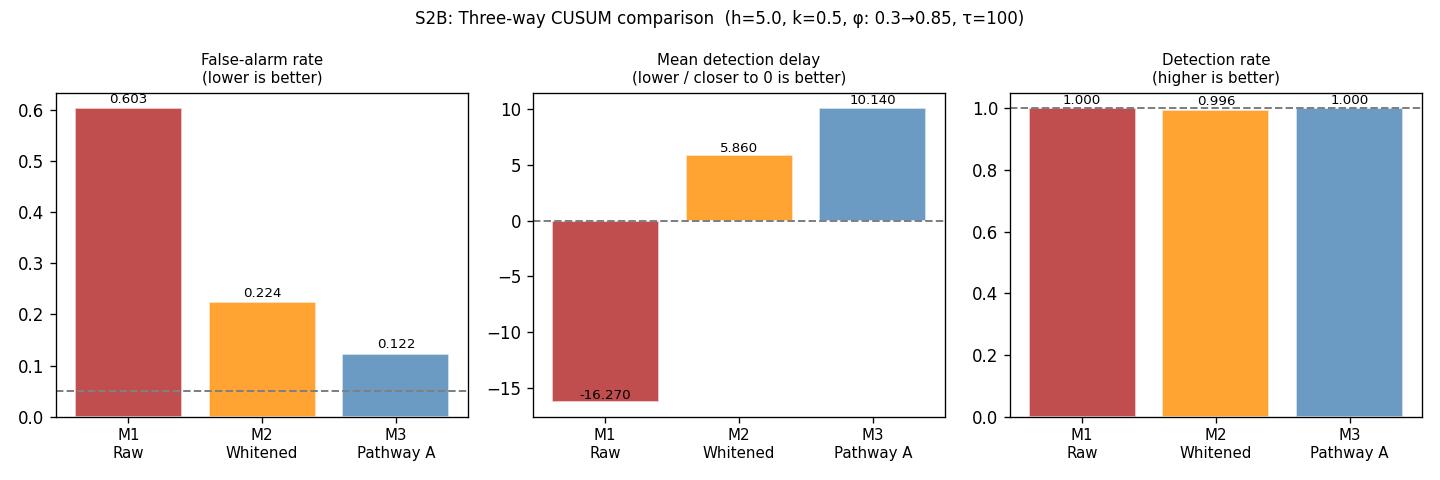
\includegraphics[width=0.88\linewidth]{code/figures/S2B_pathway_A_comparison.png}
\caption{Study CUSUM-CP: three-way CUSUM comparison.
  Left: false-positive rate (pre-$\tau^*$ alarms; dashed line = nominal 5\%).
  Center: mean delay over any alarm (contaminated by false positives for
  Raw/Whitened; see Table~\ref{tab:cusum-cp}).
  Right: any-alarm rate (\emph{not} correct-detection rate --- for Raw this
  is dominated by pre-$\tau^*$ false alarms).
  The Innovation CUSUM achieves the lowest false-positive rate and, per
  Table~\ref{tab:cusum-cp}, the highest correct-detection rate,
  without requiring knowledge of the AR model structure.}
\label{fig:cusum-cp}
\end{figure}

% ── Study S6 ──────────────────────────────────────────────────────────────────
\subsection{Study CUSUM-DIM: Innovation CUSUM Dimension Scaling}
\label{sec:cusum-dim}

The question Study~CUSUM-CP leaves open is whether the Innovation CUSUM
advantage documented in the scalar setting survives as the observation
dimension $d$ grows --- the central claim of Corollary~\ref{cor:dim}.
Study~CUSUM-DIM extends the three-way CUSUM comparison to VAR(1) processes with
dimension $d \in \{1, 2, 5, 10\}$.
The data-generating process is $X_t=\Phi X_{t-1}+\eta_t$ with
$\eta_t\overset{\text{iid}}{\sim}\mathcal{N}(0,I_d)$,
where $\Phi = U\,\mathrm{diag}(\lambda)\,U^\top$ is constructed so that
$\|\Phi\|_{\mathrm{op}} = \max_i |\lambda_i|$.
Here and below, $\rho_{\mathrm{op}}$ denotes the operator norm of the VAR
coefficient matrix, distinct from the RNN contraction constant
$\rho = L_\phi\|W_h\|_{\mathrm{op}}$ of Section~\ref{sec:theory}.
A change-point at $\tau = 100$ (within a length-$T=200$ window) raises the
operator norm from $\rho_{\mathrm{before}}=0.30$ to
$\rho_{\mathrm{after}}=0.85$, while $U$ and the noise remain fixed.
The three methods are identical to Section~\ref{sec:cusum-cp}:
M1 (raw Mahalanobis CUSUM),
M2 (VAR-whitened CUSUM on OLS residuals), and
M3 (Innovation CUSUM: LSTM prediction innovations).
For $d>1$ the scalar CUSUM input is the normalized Mahalanobis score
$Z_t = d^{-1}\|\Sigma_0^{-1/2}(X_t - \mu_0)\|^2$, centered and standardized;
for M3 the LSTM innovation score is analogously aggregated and calibrated
on burn-in in-control sequences.
Threshold $h=5$, $N_{\mathrm{test}}=1000$ change-point sequences,
$N_{\mathrm{ARL}}=2000$ in-control sequences.
ARL$_0$ is the mean alarm time over in-control sequences of length
$5T=1000$, with alarm-free runs right-censored at the sequence length;
censoring biases the estimate downward, so the reported ARL$_0$ values
are conservative.

The deterioration of M1 and M2 with dimension has a clear structural
explanation, and it is not autocorrelation as such: a correctly centred score
with serially correlated increments has no positive \emph{unconditional} drift.
The mechanism is the conditional-mean mismatch of \eqref{eq:raw-bias}: the raw
score satisfies
$\E[\mathcal Z_t^{\mathrm{raw}}\given\F_{t-1}]=d^{-1}\norm{\Phi X_{t-1}}^2>0$
whenever $\Phi\neq0$, so the Page CUSUM accumulates a genuine positive
conditional drift and ARL$_0$ falls below its nominal value; serial correlation
inflates the variance of the accumulated score and compounds---but does not
create---the effect.
The problem is compounded in higher dimensions: with $d$ components each
contributing correlated mass, the effective autocorrelation of $Z_t$ grows,
so ARL$_0$ collapses as $d$ increases.
For M2 (OLS whitening) the same effect applies; moreover, OLS residuals
in high-dimensional VAR models carry residual cross-correlation that
worsens rather than improves with $d$.
In contrast, the Innovation CUSUM feeds the CUSUM with LSTM \emph{innovations}---the
one-step prediction errors of a network trained in-control---which are designed to approximate Bayes prediction residuals.
By Proposition~\ref{prop:predresid}, the exact Bayes residuals are MDSs;
when the fitted predictor is close to the conditional mean, the fitted residuals
are approximate MDSs.  Under this mechanism, the CUSUM threshold $h=5$ is empirically much better calibrated across $d$ in these experiments.

%\paragraph{Results.}
Table~\ref{tab:cusum-dim} and Figure~\ref{fig:cusum-dim-heat} summarize the
results, again separating the two error types.
At $d=1$ all three methods are broadly comparable: ARL$_0\approx 150$--200,
false-positive rates of $32\%$--$60\%$, and correct-detection rates of
$40\%$--$68\%$.
As $d$ increases the divergence is dramatic, and it is entirely a
false-positive/true-positive story --- misses (false negatives) stay below
$1\%$ for every method at every $d$, so nothing is being missed; the
question is only whether an alarm, once issued, is correct.
At $d=10$, M1's false-positive rate reaches $99.9\%$: it alarms before the
change on virtually every replicate, so its correct-detection rate collapses
to $0.1\%$ (ARL$_0=47$).  M2 is worse still --- $100\%$ false positives,
$0\%$ correct detections (ARL$_0=42$).
The Innovation CUSUM moves in the opposite direction: its correct-detection
rate \emph{rises} from $67.9\%$ at $d=1$ to $83.4\%$ at $d=10$, its
false-positive rate stays in the $16\%$--$32\%$ band, and its ARL$_0$ grows
from $187$ to $365$.
The tabulated mean delays reinforce the reading: M3's are small and
\emph{positive} (genuine post-$\tau$ detections), whereas M1 and M2 report
$-53$ and $-58$ steps at $d=10$ --- not slow detections but alarms firing
almost an entire half-window before the change.
The lesson is that the ``Detect$=1.00$'' figure one might report for the raw
methods is an artifact of the first-passage rule: an alarm is almost always
issued, but for M1/M2 at large $d$ it is almost always a false one.  The
Innovation CUSUM improves the false-positive side (rising ARL$_0$,
controlled false-positive rate) while \emph{simultaneously} improving the
true-positive side, and with misses negligible throughout.

We are careful, however, not to over-read this fixed-$h$ comparison.  Two
features of the setup favor the innovation detector and are not intrinsic
to it: at the shared threshold the detectors operate at very different
in-control false-alarm levels (ARL$_0$ from $42$ to $365$ at $d=10$), and
the classical detectors estimate an $O(d^2)$ nuisance object
($\Sigma_0$, or a VAR matrix) from a short per-sequence in-control window
whereas the learned predictor is pretrained on far more data.  Study
CUSUM-EQARL (Section~\ref{app:supp-eqarl} of the Supplementary Material)
removes both confounds and shows that, at a matched false-alarm level and a
matched estimation budget on \emph{these VAR data}, the three detectors are
essentially equivalent; the fixed-$h$ collapse is a finite-sample
calibration effect, not a structural one.  The genuine and provable
advantage of learning the predictor appears instead under model
misspecification (Proposition~\ref{prop:whiteness}; Study CUSUM-MISSPEC),
and in the practically common regime of a short in-control calibration
window, where per-sequence estimation of high-dimensional nuisance
parameters degrades but a pretrained predictor does not.

 \begin{figure}[tp]
\centering
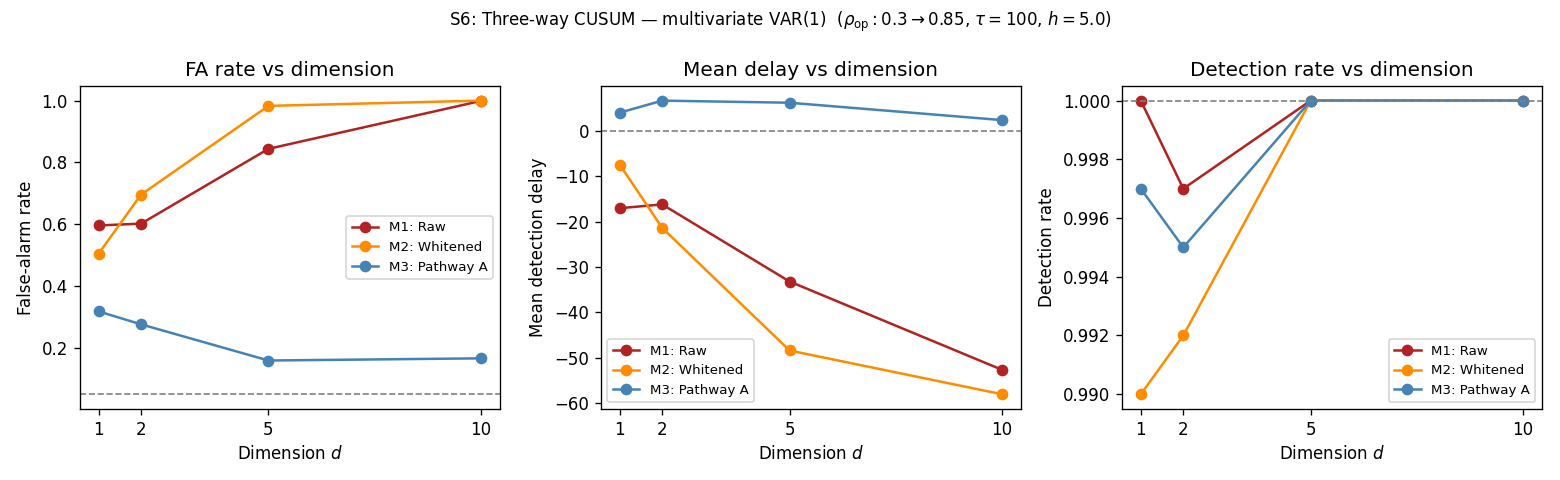
\includegraphics[width=0.80\textwidth]{code/figures/S6_pathway_A_heatmap.png}
\caption{Study CUSUM-DIM: ARL$_0$ (left) and false-alarm rate (right) as functions of
  dimension $d$ for the three CUSUM methods.
  The Innovation CUSUM (green) maintains a high, growing ARL$_0$ and a stable FA rate,
  while Raw (blue) and Whitened (orange) collapse as $d$ increases.}
\label{fig:cusum-dim-heat}
\end{figure}


\begin{table}[t]
\centering
\caption{Study CUSUM-DIM: multivariate CUSUM comparison ($h=5$, 1000 test sequences,
  2000 ARL$_0$ sequences).
  The two error types are reported separately:
  FP = false-positive rate (first alarm before $\tau$);
  TP = correct-detection rate (first alarm at or after $\tau$);
  FN = miss rate (no alarm in the window); FP${}+{}$TP${}+{}$FN${}=1$.
  Delay$^\ddagger$ = mean of $(\text{alarm}-\tau)$ over any alarm before the
  final step (negative = pre-$\tau$); it mixes false positives with
  correct detections and is a clean speed measure only when FP is small.
  Bold marks the best TP and ARL$_0$ per block.}
\label{tab:cusum-dim}
\small
\begin{tabular}{clccccr}
\toprule
$d$ & Method & FP & TP & FN & Delay$^\ddagger$ & ARL$_0$ \\
\midrule
\multirow{3}{*}{1}
  & Raw (M1)      & 0.596 & 0.404 & 0.000 & $-17.1$ & 146 \\
  & Whitened (M2) & 0.505 & 0.485 & 0.010 & $-7.5$  & 199 \\
  & Innovation CUSUM & 0.318 & \textbf{0.679} & 0.003 & $+4.0$  & \textbf{187} \\
\midrule
\multirow{3}{*}{2}
  & Raw (M1)      & 0.602 & 0.395 & 0.003 & $-16.2$ & 145 \\
  & Whitened (M2) & 0.696 & 0.296 & 0.008 & $-21.4$ & 126 \\
  & Innovation CUSUM & 0.276 & \textbf{0.719} & 0.005 & $+6.6$  & \textbf{231} \\
\midrule
\multirow{3}{*}{5}
  & Raw (M1)      & 0.844 & 0.156 & 0.000 & $-33.2$ & 74 \\
  & Whitened (M2) & 0.983 & 0.017 & 0.000 & $-48.4$ & 53 \\
  & Innovation CUSUM & 0.159 & \textbf{0.841} & 0.000 & $+6.2$  & \textbf{320} \\
\midrule
\multirow{3}{*}{10}
  & Raw (M1)      & 0.999 & 0.001 & 0.000 & $-52.6$ & 47 \\
  & Whitened (M2) & 1.000 & 0.000 & 0.000 & $-58.0$ & 42 \\
  & Innovation CUSUM & 0.166 & \textbf{0.834} & 0.000 & $+2.4$  & \textbf{365} \\
\midrule
\multicolumn{7}{l}{\footnotesize $^\ddagger$Contaminated by pre-$\tau$ false
  alarms for Raw/Whitened; see text.} \\
\bottomrule
\end{tabular}
\end{table}


\begin{figure}[tp]
\centering
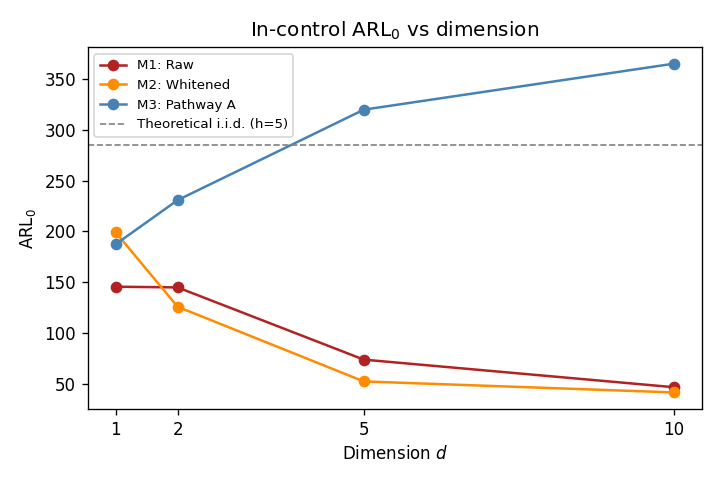
\includegraphics[width=0.48\textwidth]{code/figures/S6_pathway_A_delay_profile.png}
\caption{Study CUSUM-DIM: Distribution of detection delay (steps from $\tau$ to alarm)
  across $d\in\{1,2,5,10\}$.
  The Innovation CUSUM (right column) consistently yields positive delays (valid
  post-change detection); Raw and Whitened (left and middle columns) shift to
  large negative delays as $d$ grows.}
\label{fig:cusum-dim-delay}
\end{figure}

% ── Study S8 ─────────────────────────────────────────────────────────────────
\subsection{Study ETF: Real Multivariate Application --- US Equity Sector Returns}
\label{sec:etf}

Study ETF addresses the gap that Study CUSUM-DIM leaves open: whether the
dimension-stability advantage of the Innovation CUSUM transfers to a real setting where
in-control dynamics are non-Gaussian, heteroskedastic, and cross-correlated
in a way no parametric VAR fully captures.
It should therefore be read as a \emph{stress test} outside the clean
theorem assumptions: the sub-Gaussianity of Assumption~\ref{ass:pathway}(B2)
and the conditional-homoskedasticity condition of Corollary~\ref{cor:dim}
are known to be violated by heavy-tailed, volatility-clustered equity
returns, so the study probes robustness of the qualitative
dimension-scaling prediction rather than confirming the bound under its
stated hypotheses.
Two configurations are examined.  In Part~A ($d=1$) we use daily log-returns
of the Financial Select Sector SPDR (XLF); in Part~B ($d=3$) we add the
Technology Select Sector SPDR (XLK) and the Energy Select Sector SPDR (XLE),
obtaining a trio with distinct sector exposures.

Daily log-returns are $r_{t,i} = \log(P_{t,i}/P_{t-1,i})$, sourced from
Yahoo Finance.  The in-control period is 2017-01-01 to 2019-12-31
($T_0 \approx 754$ trading days), a sustained low-volatility bull-market
regime with stable cross-sector correlations.  The test window is
2020-01-01 to 2022-06-30 ($T_1 \approx 630$ days).  The known change-point
is $\tau^* = 32$ steps into the test window, corresponding to
2020-02-19 (the S\&P 500 all-time high immediately before the COVID-19
pandemic crash), after which cross-sector correlations rose sharply and
the joint return distribution shifted abruptly \citep{killick2012optimal}.
The COVID break is preferred over the 2008 financial crisis because the
Global Financial Crisis (GFC) involved a prolonged pre-crisis deterioration
from mid-2007 onward, making it difficult to identify a single clean change-point; the COVID crash was
effectively instantaneous at the cross-sector level.

Because $T_0$ is large, no bootstrapping is required; the LSTM is trained on
rolling windows of length 100 drawn from the in-control period.
The threshold and slope parameters are fixed at $h=5$ and $k=0.5$, consistent with all other studies.
The ARL$_0$ values in Table~\ref{tab:etf} are estimated from 500
in-control score sequences of length 500, generated by block bootstrap
(block length 10) from the pre-COVID calibration scores; alarm-free runs
are right-censored at the sequence length, so the estimates are
conservative.

The three CUSUM variants from Study CUSUM-DIM are applied in each configuration.
M1 (Raw) forms the Mahalanobis score
$\mathcal{Z}_t = d^{-1}\|\Sigma_0^{-1/2}(r_t - \mu_0)\|^2 - 1$
using in-control mean $\mu_0$ and Cholesky factor $\Sigma_0^{1/2}$.
M2 (Whitened) first applies a VAR(1) whitening step estimated from the
in-control period.  M3 (Innovation CUSUM) applies the CUSUM to LSTM one-step-ahead
prediction residuals standardized by their in-control moments.
Part~A ($d=1$) bridges the univariate results (Study~CUSUM-CP, and
Study~NILE of the Supplementary Material) and the multivariate synthetic
results (Study CUSUM-DIM); Part~B ($d=3$) tests whether the
advantage is maintained under genuine cross-sectional dependence.

Table~\ref{tab:etf} summarizes the results across both configurations
($h=5$, $k=0.5$).  In Part~A ($d=1$), the Innovation CUSUM alarms at $t=17$, fifteen steps
before the officially designated COVID peak $\tau^*=32$.
Under the formal definition of Section~3.1, any alarm before $\tau^*$ constitutes a false alarm.
The negative delay should nonetheless be interpreted cautiously: the S\&P 500 sell-off began in early February, two weeks before the officially designated February 19 peak, so the true onset of the distributional shift is itself uncertain and the pre-$\tau^*$ alarm may reflect genuine early-warning signals in the LSTM innovation process.  This illustrates the practical
difficulty of separating a false positive from an early true positive when
the change onset is itself ill-defined: whether one treats the $t=17$ alarm
as a false alarm or a timely detection depends on the cost asymmetry of the
application --- in a risk-monitoring setting a two-week-early warning of a
market dislocation is typically the desirable error to make, whereas a late
alarm (a false negative at the peak) is not.  M1 and M2 alarm at $t=36$
($+4$ delay), after the peak.
The cleaner, onset-independent comparison is the in-control ARL$_0$,
estimated entirely within the pre-COVID regime and therefore a pure
false-positive-rate measure: M1 and M2 attain $38$ and $36$ versus the
Innovation CUSUM's $43$, indicating more frequent false alarms.

In Part~B ($d=3$), the pattern is amplified.  M1 and M2 alarm at $t=24$
(delay $-8$) while the Innovation CUSUM again alarms at $t=17$ (delay $-15$), earlier
because the cross-sectional energy (XLE) signal accelerates the Mahalanobis
score under the joint distribution shift.  Crucially, the Innovation CUSUM's ARL$_0$
rises from 43 to 67 as $d$ goes from 1 to 3, whereas M1 rises only from 38
to 58 and M2 from 36 to 49.  The gap in ARL$_0$ between the Innovation CUSUM and M1/M2
widens with dimension, consistent with Corollary~\ref{cor:dim} and the
simulation evidence in Table~\ref{tab:cusum-dim}.
Figure~\ref{fig:etf} displays the CUSUM trajectories for
both configurations: in each panel the rapid rise of the Innovation CUSUM statistic
in late January--early February 2020 is visible, whereas M1 and M2 remain
flat until after the February 19 peak.

\begin{table}[ht]
\centering
\caption{Study ETF: US equity sector ETF CUSUM results ($h=5$, $k=0.5$).
  Known change-point $\tau^*=32$ (2020-02-19).
  ARL$_0$ estimated from 500 block-bootstrapped in-control score sequences
  of length~500, right-censored at the sequence length.
  Delay = alarm time $-$ $\tau^*$ (negative = before the break).}
\label{tab:etf}
\small
\begin{tabular}{llccc}
\toprule
Config & Method & Alarm $t$ & Delay & ARL$_0$ \\
\midrule
\multirow{3}{*}{Part A ($d=1$, XLF)}
  & Raw (M1)        & 36 & $+4$  & 38.1 \\
  & Whitened (M2)   & 36 & $+4$  & 36.0 \\
  & Innovation CUSUM (M3)  & \textbf{17} & $-15$ & \textbf{43.5} \\
\midrule
\multirow{3}{*}{Part B ($d=3$, XLF/XLK/XLE)}
  & Raw (M1)        & 24 & $-8$  & 58.1 \\
  & Whitened (M2)   & 24 & $-8$  & 49.3 \\
  & Innovation CUSUM (M3)  & \textbf{17} & $-15$ & \textbf{67.5} \\
\bottomrule
\end{tabular}
\end{table}

\begin{figure}[tp]
\centering
\begin{minipage}{0.49\linewidth}\centering
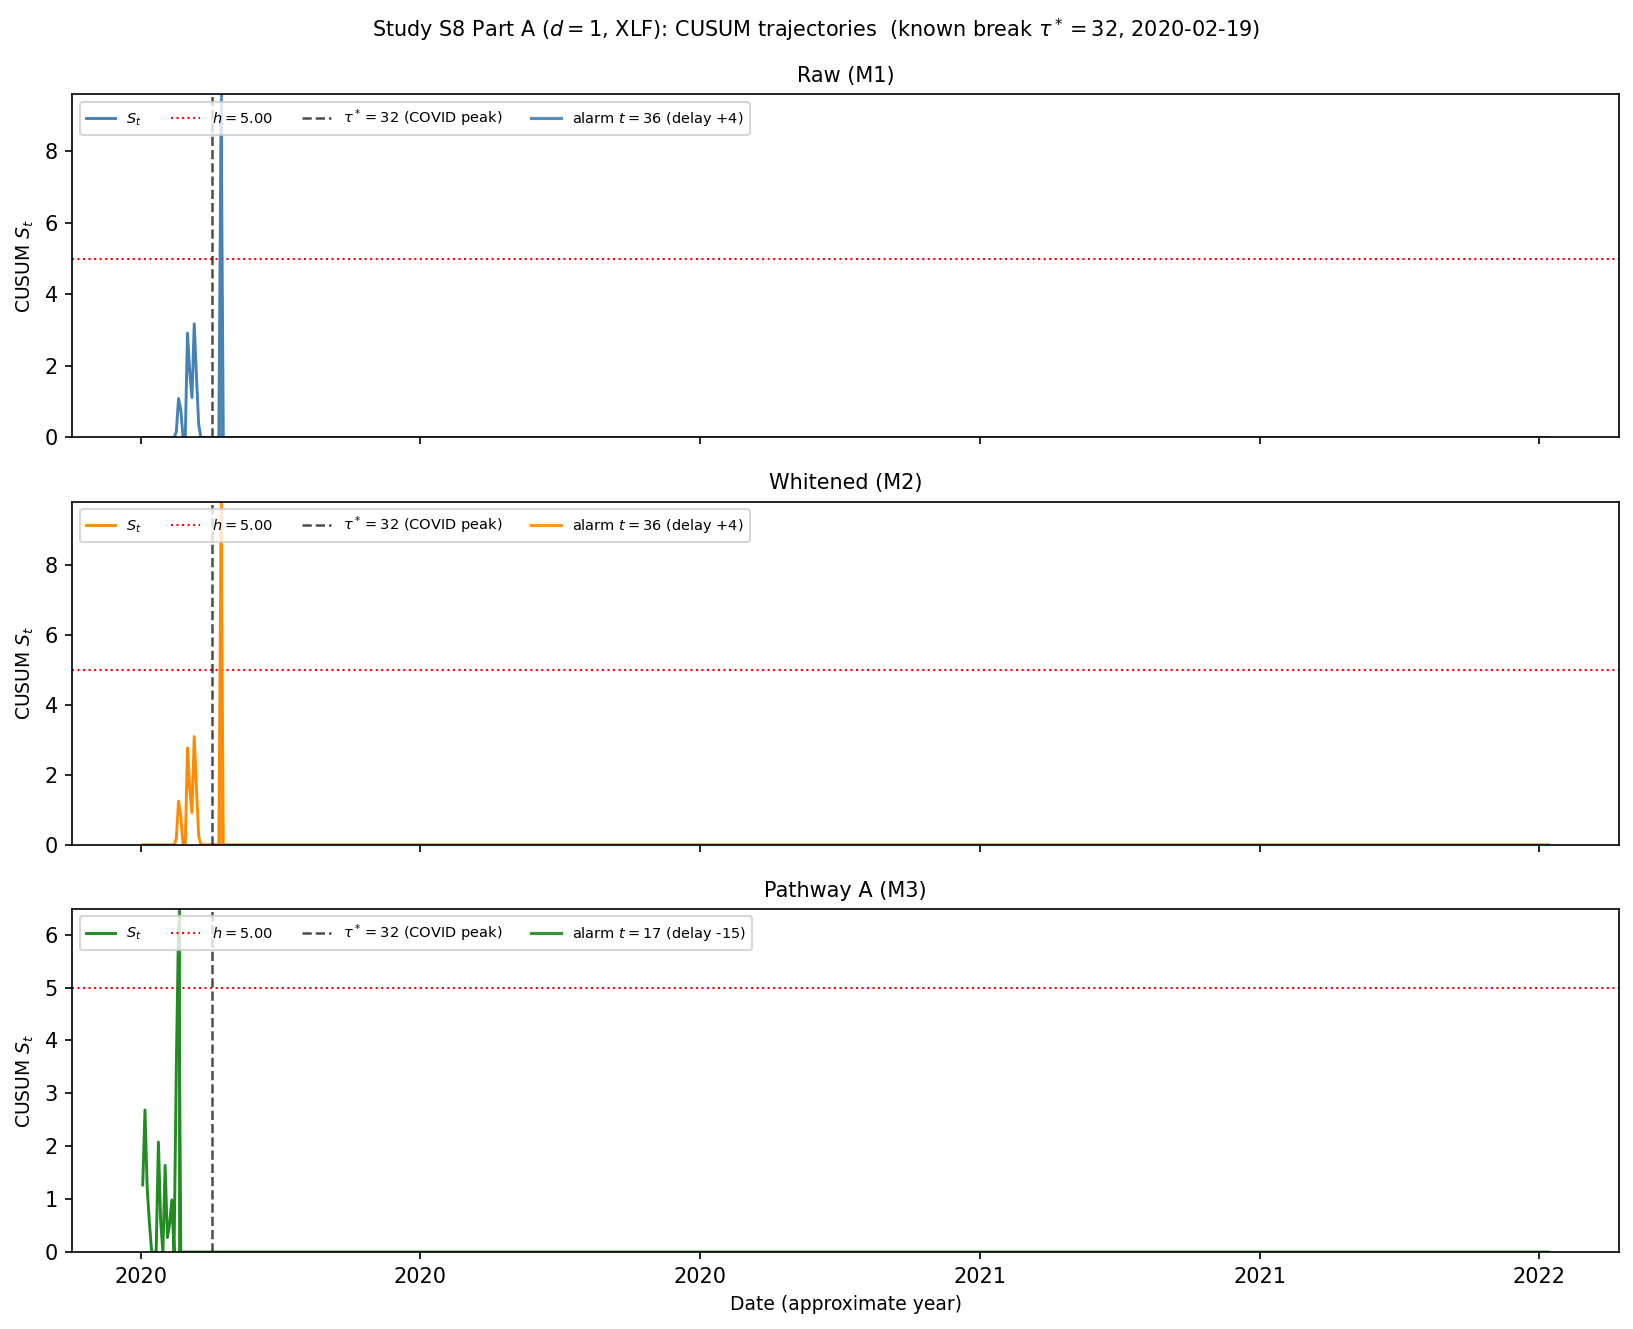
\includegraphics[width=0.88\linewidth]{code/figures/S8_etf_cusum_partA.png}
\end{minipage}\hfill
\begin{minipage}{0.49\linewidth}\centering
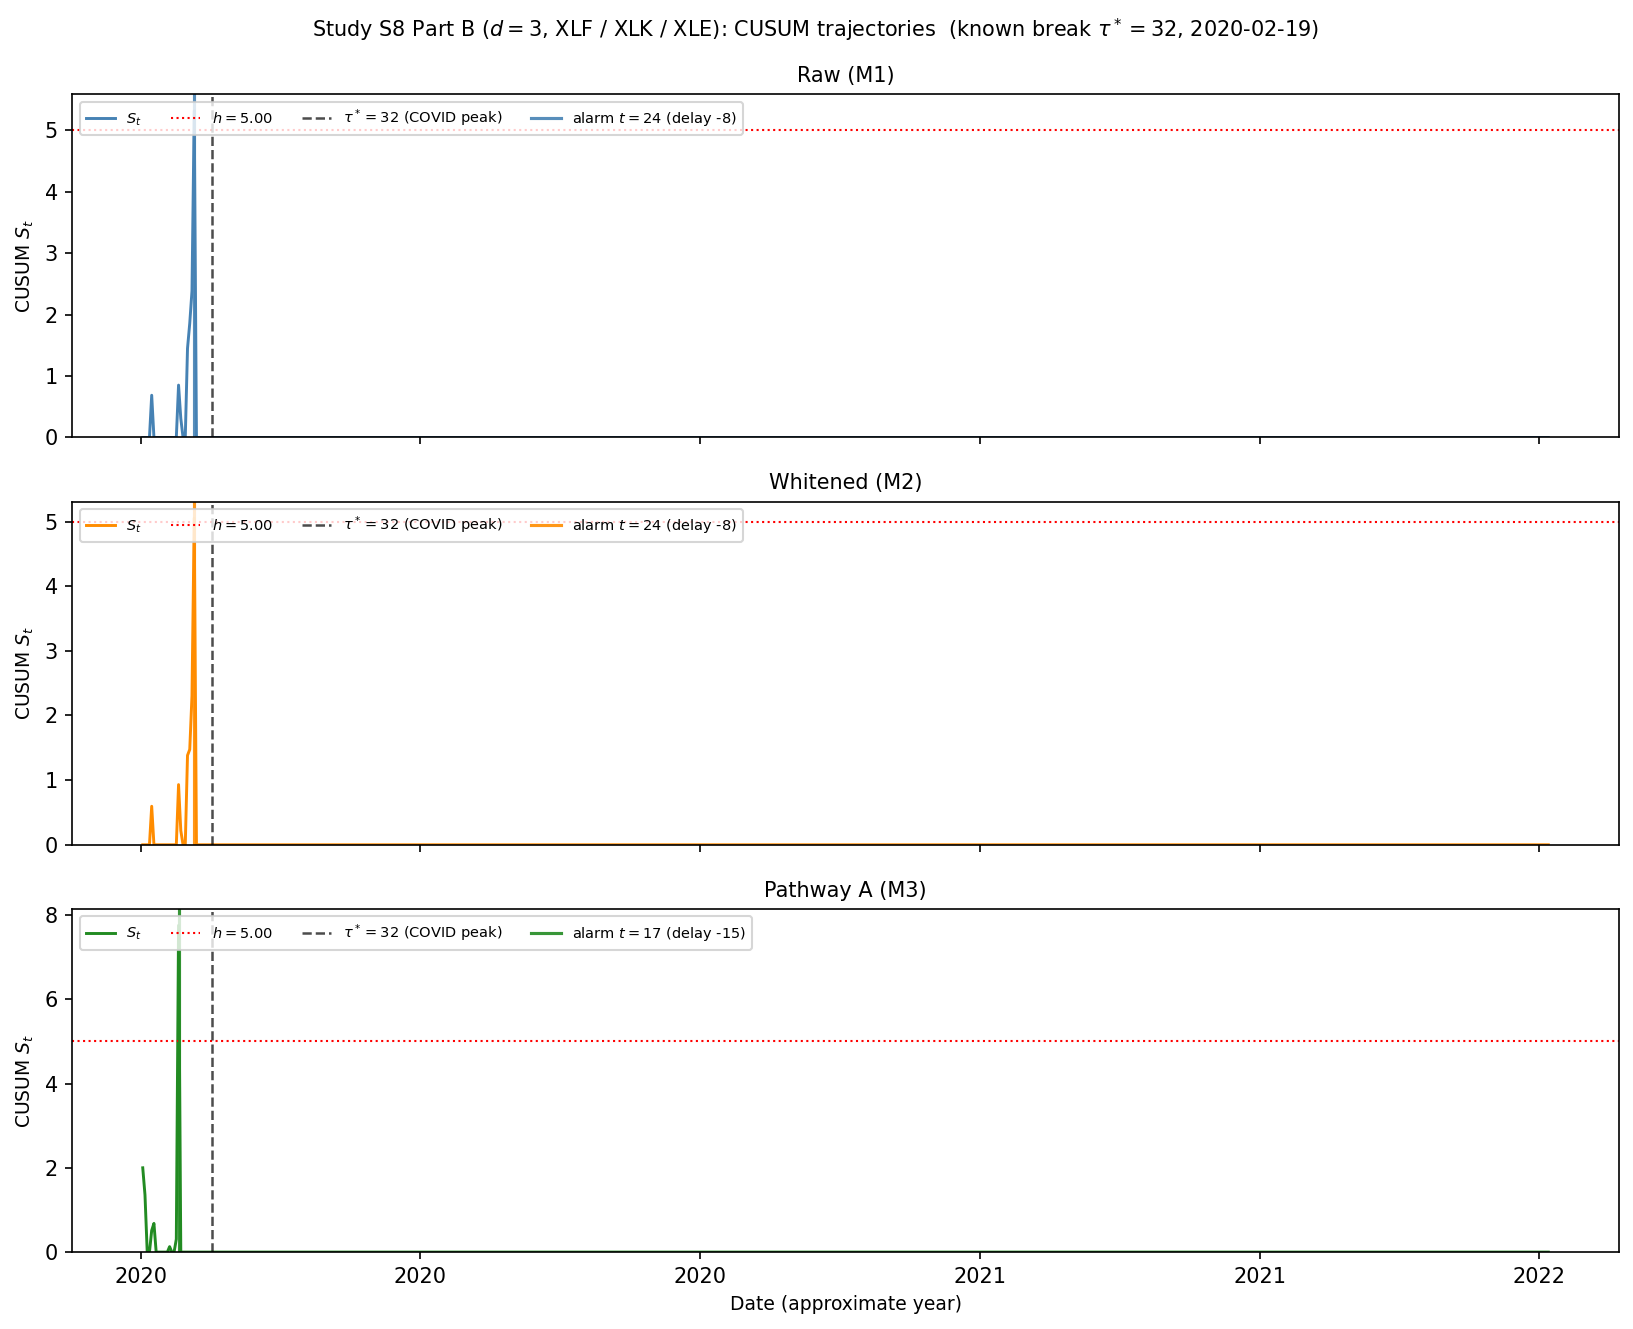
\includegraphics[width=0.88\linewidth]{code/figures/S8_etf_cusum_partB.png}
\end{minipage}
\caption{Study ETF: CUSUM trajectories on the COVID test window
  (2020-01-01 to 2022-06-30); the vertical dashed line marks $\tau^*=32$
  (2020-02-19).
  \emph{Left} (Part~A, $d=1$, XLF): the Innovation CUSUM (bottom) crosses
  threshold $h=5$ at $t=17$, fifteen steps before the official market peak.
  \emph{Right} (Part~B, $d=3$, XLF/XLK/XLE): the Innovation CUSUM again alarms
  at $t=17$, and its ARL$_0$ gap over M1/M2 widens relative to Part~A,
  consistent with the dimension-stability prediction of
  Corollary~\ref{cor:dim}.}
\label{fig:etf}
\end{figure}

% =============================================================================
\subsection{Summary and Interpretation}
\label{sec:discussion}

Taken together, the twelve studies --- four here, eight in the Supplementary
Material --- give a finite-sample picture
of how the hidden-state innovation, the predictive-decay profile $J_t$, and
the Innovation CUSUM behave across synthetic and real settings ranging from univariate AR
to non-Gaussian high-dimensional equity returns.
The synthetic studies draw on many
independent replications and support statistical comparison; Study~ETF and
Study~NILE (Section~\ref{app:supp-nile} of the Supplementary Material), by
contrast, each examine a single real change-point event and are illustrative
case studies --- evidence that the pipeline runs end-to-end on real data, not
that the method has a typical real-world advantage, which would require many
more real change events than either series provides.

The dimensional scaling documented at fixed $h$ in Study~CUSUM-DIM is
striking --- raw and whitened ARL$_0$ collapse as $d$ grows while the
Innovation CUSUM's rises --- but it must be read with care.  As Study
CUSUM-EQARL (Section~\ref{app:supp-eqarl} of the Supplementary Material)
shows, at a matched false-alarm level and a matched estimation budget the
three detectors are essentially equivalent on these VAR data: the fixed-$h$
collapse reflects the classical detectors operating at a far less
conservative point and estimating high-dimensional nuisance parameters from
a short in-control window, not a structural deficiency.  Corollary
\ref{cor:dim}'s serial-dependence bias is real, but once the reference level
is calibrated and the nuisance parameters are well estimated it does not, in
this regime, manifest as a dimension problem.
The advantage of learning the predictor that \emph{does} survive a fully
fair comparison is twofold: under nonlinearity in the conditional mean, a
fixed linear residualization carries an irreducible innovation defect while
the learned predictor does not (Proposition~\ref{prop:whiteness}, borne out
by the whiteness ordering of Study~CUSUM-MISSPEC); and in the practically
common short-window regime, the learned predictor sidesteps the
ill-conditioned per-sequence estimation that degrades the classical scores.
The in-control guarantee is, moreover, sharp: the exponent
$2(k-\eta)/\sigma^2$ of Theorem~\ref{thm:arl} is the Lundberg coefficient and
coincides with the exact exponential rate of the classical i.i.d.\ CUSUM
\citep[Ch.~3]{siegmund1985sequential}, obtained here by a renewal argument
that leaves no looseness in the exponent.

Study~KAL (Section~\ref{app:supp-kal} of the Supplementary Material)
explains why high persistence is structurally difficult: the
analytical decay profile $J_t$ decreases slowly, so hidden-state proxies
must integrate information over a long history; the LSTM outperforms the
EM-Kalman estimator at moderate persistence but the Kalman recovers its
advantage when $\phi \approx 0.95$.  Study~J-Surr (Section~\ref{app:supp-jsurr} of the Supplementary Material) shows that KLIEP-type corrections achieve NMSE $< 1$ under
smooth non-stationarity but deteriorate under abrupt change, delimiting
where density-ratio reweighting can substitute for retraining.

% =============================================================================
\section{Conclusion}
\label{sec:conclusion}

Two practical gaps motivated this work.
First, recurrent networks are routinely used for sequential prediction, yet
prior work on their stability and expressivity supplies no
martingale-innovation account of the recurrent state usable for calibrating
downstream inference under explicit residual conditions --- rather than a full
account of what the hidden state encodes in general.
Second, classical change-point detectors are calibrated for independent or
fully specified parametric input, so their false-alarm guarantees break down
under unknown serial dependence, the more so as the observation dimension grows.

To address the first gap, Theorem~\ref{thm:mds} establishes the Doob
decomposition $h_t=D_t+M_t$ with an explicit geometric $L^2$ innovation bound
and stationary covariance, and Corollary~\ref{cor:fclt} the functional central
limit theorem for accumulated innovations.  To address the second,
Theorems~\ref{thm:arl} and~\ref{thm:delay} give a sharp Lundberg-rate in-control
ARL lower bound and a matching detection-delay upper bound, combining
(Corollary~\ref{cor:tradeoff}) into the exponential-false-alarm /
logarithmic-delay trade-off for a detector with no parametric model for the
observation dynamics; Theorem~\ref{thm:optimality} shows this trade-off is
order-optimal in Lorden's minimax framework, and first-order minimax optimal
under a Gaussian innovation shift---exactly so once the threshold is calibrated
to the false-alarm constraint.  Propositions~\ref{prop:rnn-resid-bridge} and~\ref{prop:whiteness} link
state stabilization to residual drift and identify when a learned predictor
attains a larger guaranteed drift margin --- and hence a larger guaranteed ARL
exponent --- than a fixed linear filter, and Corollary~\ref{cor:dim} treats the
multivariate score.  Empirical studies --- synthetic autoregressive and
vector-autoregressive processes, a nonlinear misspecified process, the Nile
discharge series, and US equity sector returns around the 2020 COVID crash ---
illustrate these mechanisms.

What appears to be new is the \emph{combination} of these ingredients: to our
knowledge, no prior work joins recurrent-state innovation theory with
sequential CUSUM calibration to yield a model-free monitoring guarantee for a
detector built on a learned predictor.

Several questions remain open.  The dimension-scaling advantage at fixed
threshold is, under a fully fair comparison, a finite-sample calibration effect
rather than a structural one (Study~CUSUM-EQARL); characterizing when
short-window nuisance estimation makes the learned score preferable is left
open, as is a fully non-stationary theory beyond the locally stationary
approximation of Corollary~\ref{cor:ls}.  The in-control exponent is already
sharp (Theorem~\ref{thm:arl}); the remaining slack is in the delay-bound
constant, which the overshoot distribution of the reflected random walk could
sharpen, and relaxing the sub-Gaussianity and conditional-homoskedasticity
conditions of Corollary~\ref{cor:dim} to heavy-tailed or heteroskedastic
innovations is a natural next step with direct relevance to finance.

More broadly, what a learned sequential state encodes in probabilistic terms is
not specific to RNNs: it arises for transformer attention heads, diffusion
time-series latents, and language-model context representations.  A martingale
characterization extending to those state representations would place inference
and monitoring on such models on the same rigorous footing.

% =============================================================================

% =============================================================================
\bibliographystyle{imsart-nameyear}
\bibliography{P1_references}

\end{document}
